\newcommand{\GCNetname}{Guided Calibration Network\xspace}
\newcommand{\gcnetname}{guided calibration network\xspace}
\newcommand{\gcnetacronymnospace}{GCNet}
\newcommand{\gcnetacronym}{\gcnetacronymnospace\xspace}
\newcommand{\gbr}{GBR\xspace}
\newcommand{\LCNetreg}{LCNet$_\text{reg}$\xspace}

\chapter{Learning Lighting Calibration for Photometric Stereo}
\label{ch:lcnet}

\section{Introduction}
Photometric stereo aims at recovering the surface normal of a static object from a set of images captured under different light directions~\cite{woodham1980ps,silver1980determining}. \emph{Calibrated} photometric stereo methods assume known light directions, and promising results have been reported~\cite{shi2019benchmark} at the cost of tedious light source calibration. The problem of \emph{uncalibrated} photometric stereo, where light directions are unknown, still remains an open challenge, and its stable solution is wanted because of the ease of setting. In this chapter, we study the problem of uncalibrated photometric stereo for surfaces with general and unknown isotropic reflectance.

Most of the existing methods for uncalibrated photometric stereo~\cite{alldrin2007r,shi2010self,papad14closed} assume a simplified reflectance model, such as the Lambertian model, and focus on resolving the shape-light ambiguity, such as the Generalized Bas-Relief (GBR) ambiguity~\cite{belhumeur1999bas}. Although methods of~\cite{lu2013uncalibrated,lu2015uncalibrated} can handle surfaces with general bidirectional reflectance distribution functions (BRDFs), they rely on a uniform distribution of light directions for deriving a solution.

Recently, with the great success of deep learning in various computer vision tasks, deep learning based methods have been introduced to calibrated photometric stereo~\cite{santo2017deep,Taniai18,ikehata2018cnn,chen2018ps}. Instead of explicitly modeling complex surface reflectances, they directly learn the mapping from reflectance observations to surface normals given light directions. Although they have produced promising results in a calibrated setting, they cannot handle the more challenging problem of \emph{uncalibrated} photometric stereo, where light directions and intensities are unknown. One simple strategy to handle uncalibrated photometric stereo with deep learning is to directly learn the mapping from images to surface normals without taking the light directions as input. 
However, as reported in~\Sref{sub:upsfcn}, the performance of such a model lags far behind those which take both images and light directions as input.

Instead of directly predicting surface normals from images, we propose to first estimate light directions and intensities from images. The problem of uncalibrated photometric stereo can then be reduced to a calibrated one, which can be effectively solved by existing calibrated methods~\cite{shi2014bi,chen2018ps,ikehata2018cnn}.
The rationales behind this two-stage approach are as follows. First, lighting information is very important for normal estimation since lighting is the source of various cues, such as shading and reflectance, and estimating the light directions ($3$-vectors) and intensities (scalars) is in principle much easier than directly estimating the normal map (a $3$-vector at each pixel location) together with the lighting conditions. 
Second, by explicitly learning to estimate light directions and intensities, the model can take advantage of the intermediate supervision by the ground-truth lighting, resulting in a more interpretable behavior. 

This work focuses on learning lighting calibration for uncalibrated photometric stereo. The contributions of this work can be summarized as follows:
\begin{itemize}
    \item We introduce a lighting calibration network, named LCNet, for estimating light directions and intensities from images.
    \item We discuss the differences between LCNet and traditional uncalibrated methods, and analyze the features learned by LCNet to resolve the \gbr ambiguity.
    \item We find that attached shadows, shadings, and specular highlights are key elements for lighting estimation, and that LCNet extracts features independently from each input image without exploiting any inter-image information (``inter-image'' means information shared by all images).
    \item Based on our findings, we propose a \gcnetname (\gcnetacronym) that explicitly utilizes object shape and shading information as guidances for better lighting estimation.
\end{itemize}

Preliminary results of this research have been published in~\cite{chen2019self,chen2020chen_gcnet}.
Our code and models can be found at \url{https://guanyingc.github.io/SDPS-Net}.

\section{Related Work}
\label{sec:lcnet_relatedwork}
In this section, we review uncalibrated photometric stereo methods and the loosely related work on learning based lighting estimation. Review for recent deep calibrated photometric stereo methods can be found in~\Sref{sec:psfcn_related_work}.

\paragraph{Uncalibrated photometric stereo}
When lighting is unknown, the surface normals of a Lambertian object can only be estimated up to a $3\times 3$ linear ambiguity~\cite{hayakawa1994photometric}, which can be reduced to a $3$-parameter GBR ambiguity~\cite{belhumeur1999bas,yuille1999determining} using the surface integrability constraint. Previous work used additional clues like albedo priors~\cite{alldrin2007r,shi2010self}, inter-reflections~\cite{chandraker2005reflections}, specular spikes~\cite{drbohlav2005can}, Torrance and Sparrow reflectance model~\cite{georghiades2003incorporating}, reflectance symmetry~\cite{tan2007isotropy,wu2013calib}, multi-view images~\cite{esteban2008multiview}, and local diffuse maxima~\cite{papad14closed}, to resolve the GBR ambiguity. Cho~\etal~\cite{cho2016photometric} considered a semi-calibrated case where the light directions are known but not their intensities. There are few works that can handle non-Lambertian surfaces under unknown lighting. Hertzmann and Seitz~\cite{hertzmann2005example} proposed an exemplar based method by inserting an additional reference object to the scene. Methods based on cues like similarity in radiance changes~\cite{sato2007shape,lu2013uncalibrated} and attached shadow~\cite{okabe2009attached} were also introduced, but they require the light sources to be uniformly distributed on the entire viewing sphere. Recently, Lu~\etal~\cite{lu2018symps} introduced a method based on the ``constrained half-vector symmetry'' to work with non-uniform lightings. Different from these traditional methods, our method can deal with surfaces with general and unknown isotropic reflectance without the need of explicitly utilizing any additional clues or reference objects, solving a complex optimization problem at test time, or making assumptions on the light source distribution. 

Other methods related to uncalibrated photometric stereo include exemplar-based methods~\cite{hertzmann2005example}, regression-based methods~\cite{midorikawa2016uncalibrated}, semi-calibrated photometric stereo~\cite{cho2018semi}, inaccurate lighting refinement~\cite{queau2017non}, and photometric stereo under general lighting~\cite{basri2007photometric,mo2018uncalibrated,haefner2019variational}.

\paragraph{Learning based lighting estimation}
Recently, learning based single-image lighting estimation methods have attracted considerable attention. Gardner~\etal~\cite{gardner2017learning} introduced a CNN for estimating HDR environment lighting from an indoor scene image. Hold-Goeffroy~\etal~\cite{hold2017deep} learned outdoor lighting using a physically-based sky model. Weber~\etal~\cite{weber2018learning} estimated indoor environment lighting from an image of an object with known shape. Zhou~\etal~\cite{Zhou_2018_CVPR} estimated lighting, in the form of Spherical Harmonics, from a human face image by assuming a Lambertian reflectance model. Different from the above methods, our method can estimate accurate directional lightings from multiple images of a static object with general shape and non-Lambertian surface.

\section{Lighting Calibration Network (LCNet)}
\label{sec:lcnet}
In the rest of this chapter, we refer to light direction and intensity as ``lighting''.
To estimate lighting from the images, an intuitive approach would be directly regressing the light direction vectors and intensity values.
However, we propose that formulating the lighting estimation as a classification problem is a superior choice, as will be verified by our experiments. Our arguments are as follows. First, classifying a light direction into a certain range is easier than regressing the exact value(s), and this will reduce the learning difficulty. 
Second, when training a normal estimation network, taking discretized light directions as input will allow it to better tolerate small errors in the estimated light directions.

\begin{figure}[htbp] \centering
    \tdplotsetmaincoords{70}{105}
\pgfmathsetmacro{\rvec}{1}
\pgfmathsetmacro{\thetavec}{40}
\pgfmathsetmacro{\phivec}{45}
\begin{tikzpicture}[scale=2.0,tdplot_main_coords]
    \coordinate (O) at (0,0,0); %
    \draw[->] (0,0,0) -- (1,0,0) node[below=0.5ex,left=-0.4ex]{$z$};
    \draw[->] (0,0,0) -- (0,1,0) node[right=-0.4ex]{$x$};
    \draw[->] (0,0,0) -- (0,0,1) node[above=-0.4ex]{$y$};
    \draw[dashed,color=gray] (0,0,0) -- (0,0,-1);
    \draw[dashed,color=gray] (0,0,0) -- (0,-1,0);
    \tdplotdrawarc[dashed,color=gray]{(O)}{1}{-90}{90}{}{}
    \tdplotsetthetaplanecoords{0}
    \tdplotdrawarc[semithick,dashed,color=gray,tdplot_rotated_coords]{(0,0,0)}{1}{0}{180}{}{}
    \tdplotsetthetaplanecoords{90}
    \tdplotdrawarc[semithick,dashed,color=gray,tdplot_rotated_coords]{(0,0,0)}{1}{0}{360}{}{}

    \tdplotsetcoord{P}{\rvec}{\thetavec}{\phivec} %
    \draw[line width=1pt,-stealth,color=black] (O) -- (P) node[above right] {$P$};

    \tdplotsetcoord{Px}{\rvec}{90}{\phivec} %
    \draw[dashed, color=black] (O) -- (Px);
    \tdplotdrawarc[thick,color=red]{(O)}{0.4}{\phivec}{90}{color=red,below=0.4ex,right=-0.4ex}{$\phi$} 

    \tdplotsetthetaplanecoords{\phivec} %
    \tdplotdrawarc[tdplot_rotated_coords,thick,color=blue,opacity=0.8]{(0,0,0)}{0.4}{\thetavec}{90}{above=0.4ex,right=-0.5ex}{$\theta$}
    \tdplotdrawarc[semithick,dashed,color=gray,tdplot_rotated_coords]{(0,0,0)}{1}{0}{180}{}{}
\end{tikzpicture}

    \raisebox{0.05\height}{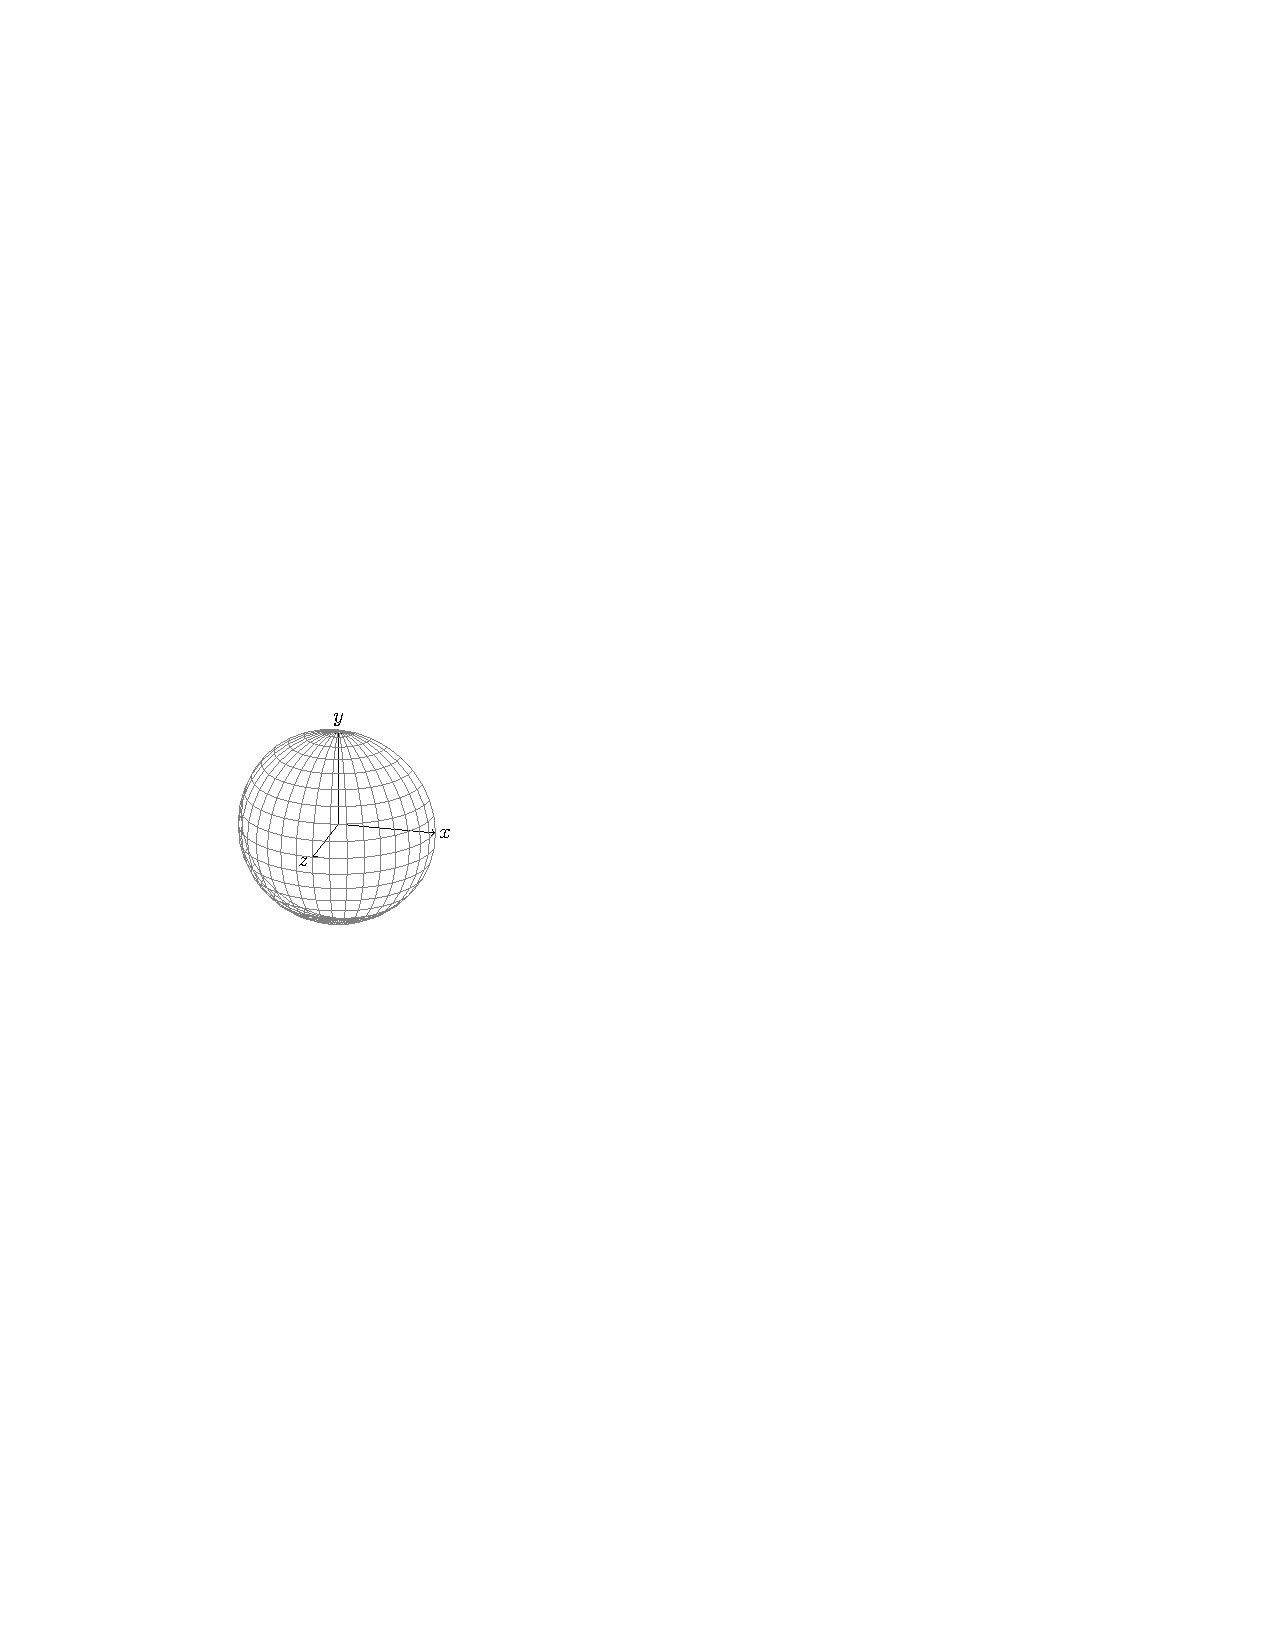
\includegraphics[width=0.28\textwidth]{ch-lcnet/images/Method/hemisphere.pdf}} \\ \vspace{-0.9em} 
    \makebox[0.28\textwidth]{\small (a)} 
    \makebox[0.28\textwidth]{\small (b)} \\
    \caption[Illustration of an example discretization of the lighting space]{(a) Illustration of the coordinate system ($z$ axis is the viewing direction). $\phi \in [0\degree, 180\degree]$ and $\theta \in [-90\degree, 90\degree]$ are the azimuth and elevation of the light direction, respectively. (b) Example discretization of the light direction space when $K_d=18$.} \label{fig:coord}
\end{figure}

\subsection{Discretization of Lighting Space} Since we cast our lighting estimation as a classification problem, we need to discretize the continuous lighting space. Note that a light direction in the upper-hemisphere can be described by its azimuth $\phi \in [0\degree, 180\degree]$ and elevation $\theta \in [-90\degree, 90\degree]$ (see \fref{fig:coord}~(a)). We can discretize the light direction space by evenly dividing both the azimuth and elevation into $K_d$ bins, resulting in $K_d^2$ classes (see \fref{fig:coord}~(b)). Solving a $K_d^2$-class classification problem is not computationally efficient, as the softmax probability vector will have a very high dimension even when $K_d$ is not large (\eg, $K_d^2=1,296$ when $K_d=36$). 
Instead, we estimate the azimuth and elevation of a light direction separately, leading to two $K_d$-class classification problems. Similarly, we evenly divide the range of possible light intensities into $K_e$ classes (\eg, $K_e=20$ for a possible light intensity range of $[0.2, 2.0]$).

\begin{figure}[htbp] \centering
	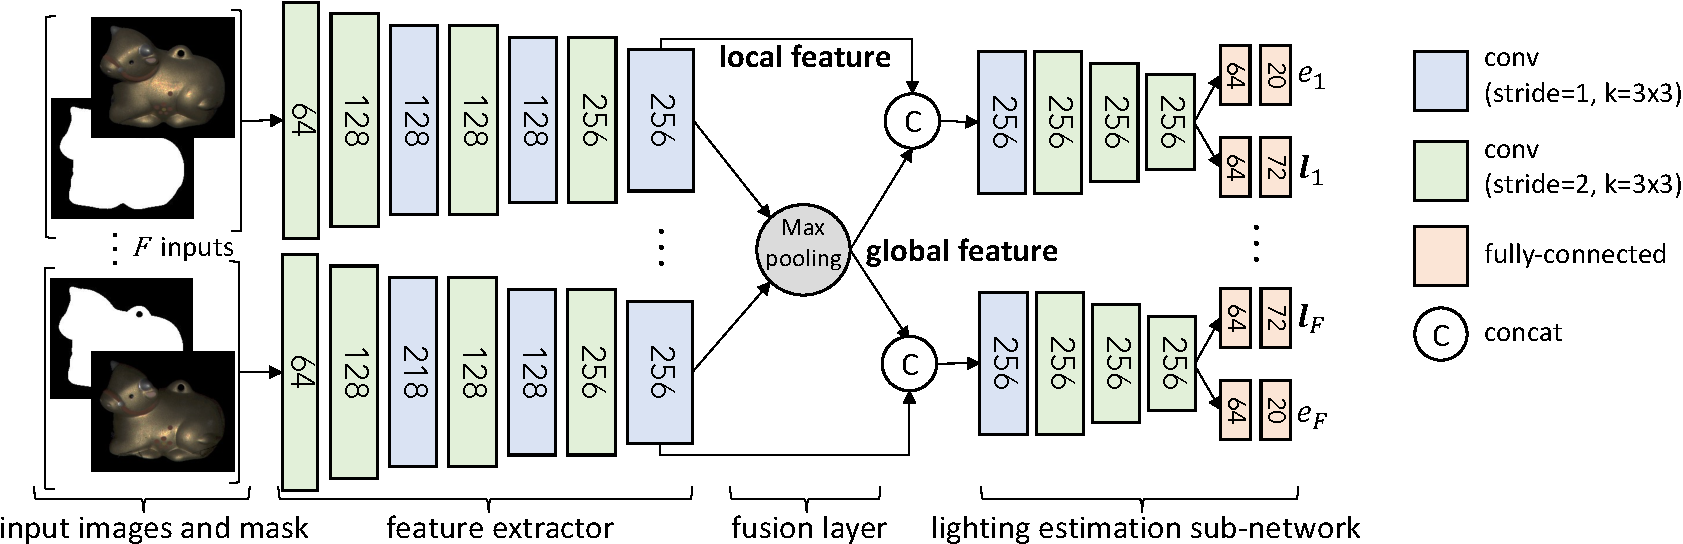
\includegraphics[width=1\textwidth]{ch-gcnet/images/Method/LCNet.pdf}
    \caption[Network architecture of LCNet]{Network architecture of LCNet. Each layer's value indicates its output channel number.} \label{fig:LCNet}
\end{figure}

\subsection{Local-global Feature Fusion}
A straightforward approach to estimate the lighting for each image is simply taking a single image as input, encoding it into a feature map using a CNN, and feeding the feature map to a lighting prediction layer. It is not surprising that the result of such a simple solution is far from satisfactory. Note that the appearance of an object is determined by its surface geometry, reflectance model and the lighting. The feature map extracted from a single observation obviously does not provide sufficient information for resolving the shape-light ambiguity. Thanks to the nature of photometric stereo where multiple observations of an object are considered, we propose a local-global feature fusion strategy to extract more comprehensive information from multiple observations.

Specifically, we separately feed each image into a shared-weight feature extractor to extract a feature map, which we call \emph{local feature} as it only provides information from a single observation. All local features of the input images are then aggregated into a \emph{global feature} through a max-pooling operation, which has been proven to be efficient and robust on aggregating salient features from a varying number of unordered inputs~\cite{wiles2017silnet,chen2018ps}. Such a global feature is expected to convey implicit surface geometry and reflectance information of the object which help resolve the ambiguity in lighting estimation. Each local feature is concatenated with the global feature, and fed to a shared-weight lighting estimation sub-network to predict the lighting for each individual image. By taking both local and global features into account, our model can produce much more reliable results than using the local features alone. We empirically found that additionally including the object mask as input can effectively improve the performance of lighting estimation, as will be seen in the experiment section.

\subsection{Network Architecture}
LCNet is a multi-input-multi-output (MIMO) network that consists of a shared-weight \emph{feature extractor}, an \emph{aggregation layer} (\ie, max-pooling layer), and a shared-weight \emph{lighting estimation sub-network} (see \fref{fig:LCNet}). 
It takes the observations of the object together with the object mask as input, and outputs the light directions and intensities in the form of softmax probability vectors of dimension $K_d$ (azimuth), $K_d$ (elevation) and $K_e$ (intensity), respectively. 
We convert the output of LCNet to $3$-vector light directions and scalar intensity values by simply taking the middle value of the range with the highest probability. We have experimentally verified that alternative ways like taking the expectation of the probability vector or performing quadratic interpolation in the neighborhood of the peak value do not improve the result.

\paragraph{Loss function}
Multi-class cross entropy loss is adopted for both light direction and intensity estimation, and the overall loss function is
\begin{align}
    \label{eq:cls_loss}
    \mathcal{L}_{\text{Light}} & = \lambda_{l_a} \mathcal{L}_{l_a} + \lambda_{l_e} \mathcal{L}_{l_e} + \lambda_e \mathcal{L}_e,
\end{align}
where $\mathcal{L}_{l_a}$ and $\mathcal{L}_{l_e}$ are the loss terms for azimuth and elevation of the light direction, and $\mathcal{L}_e$ is the loss term for light intensity. 
For example, given $F$ input images,
\begin{align}
    \label{eq:cls_detail_loss}
    \mathcal{L}_{l_a}=-\frac{1}{F} \sum_{f=1}^{F} \sum_{i=1}^{K_d} \{y_{i}^f=1\} \log(p_i^f),
\end{align}
where $\{\cdot\}$ is a binary indicator (0 or 1) function, $y_i^f$ is the ground-truth label ($0$ or $1$) and $p_i^f$ is the predicted probability for bin $i$ ($K_d$ bins in our case) for the $f$\textsuperscript{th} image. Detailed definition of other loss terms are similar to \eref{eq:cls_detail_loss}.
During training, weights $\lambda_{l_a}$, $\lambda_{l_e}$, and $\lambda_e$ for the loss terms are set to $1$.


\subsection{Training Data}
We adopted the synthetic Blobby and Sculpture datasets introduced in~\Sref{sec:psfcn_dataset} for training.
Blobby and Sculpture datasets provide surfaces with complex normal distributions and diverse materials from MERL dataset~\cite{matusik2003merl}. Effects of cast shadow and inter-reflection were considered during rendering using the physically based raytracer Mitsuba~\cite{jakob2010mitsuba}. There are $85,212$ samples in total. Each sample was rendered under $64$ distinct light directions sampled from the upper-hemisphere with uniform light intensity, resulting in $5,453,568$ images ($85,212 \times 64$). The rendered images have a dimension of $128\times 128$.

To simulate images under different light intensities, we randomly generated light intensities in the range of $[0.2, 2.0]$ to scale the magnitude of the images (\ie, the ratio of the highest light intensity to the lowest one is $10$)\footnote{Note that the ratio (other than the exact value) matters, since light intensity can only be estimated up to a scale factor.}. Note that this selected range contains a wider range of intensity value than the public photometric stereo datasets like \diligent~\cite{shi2019benchmark} and \gourd~\cite{alldrin2008p}. The color intensities of the input images were normalized to the range of $[0, 1]$. 
During training, we applied noise perturbation in the range of $[-0.025, 0.025]$ for data augmentation, and the input image size for LCNet was $128\times 128$. At test time, the input for LCNet is rescaled to $128\times 128$ as it contains fully-connected layers and requires the input to have a fixed spatial dimension. Trained only on the synthetic dataset, we will show that our model can generalize well on real datasets.

\paragraph{Implementation details}
Our method was implemented in PyTorch~\cite{paszke2017pytorch} and Adam optimizer~\cite{kingma2014adam} was used with default parameters. LCNet contains $4.4$ million parameters.
We trained LCNet using a batch size of $32$ for $20$ epochs, and the learning rate was initially set to $0.0005$ and halved every $5$ epochs.
It took about $22$ hours to train LCNet on a single Titan X Pascal GPU with a fixed input image number of $32$.

\subsection{Evaluation of LCNet with Synthetic Data}
\label{sub:eval_lcnet}
We evaluate LCNet on the synthetic test dataset \syntestMERL introduced in \Sref{subsec:synth_test_data}.
To measure the accuracy of the predicted light directions, the widely used mean angular error (MAE) in degree is adopted.
Since the light intensities among the testing images can only be estimated up to a scale factor $s$, we introduce the scale-invariant relative error (RE)
\begin{equation}
    RE_{scale} = \frac{1}{q} \sum_i^q \left(\frac{|s e_i -\tilde{e}_i|}{\tilde{e}_i} \right),
\end{equation}
where $q$ is the number of images, $e_i$ and $\tilde{e}_i$ are the estimated and ground-truth light intensities, respectively, for image $i$. The scale factor $s$ is computed by solving \hbox{$\argmin_s \sum_i^n (s e_i -\tilde{e}_i)^2$} with least squares. 
As the calibrated intensity in the real dataset is in the form of a $3$-vector, we repeat the estimated intensity to form a $3$-vector and calculate the average result.

For all experiments on synthetic dataset involving input with unknown light intensities, we randomly generated light intensities in the range of $[0.2, 2.0]$. Each experiment was repeated five times and the average results were reported.

\paragraph{Discretization of lighting space}
For a given number of bins $K_d$, the maximum deviation angle for azimuth and elevation of a light direction is $\delta = 180\degree/(K_d\times 2)$ after discretization (\eg, $\delta=2.5\degree$ when $K_d=36$).
Note that discretizing azimuth and elevation angles independently indicates that lighting space is more densely discretized around the poles and less around the equator. 
This suggests that the link between the quantization of the lighting space and surface normal estimation error correlates with the lighting distribution.
To investigate how the light direction discretization affects the surface normal estimation accuracy, we tested PS-FCN on \emphobject{Sphere} and \emphobject{Bunny} rendered under three different lighting distributions, namely, \textit{Near Uniform}, \textit{Around Equator}, and \textit{Around Poles} (see \fref{fig:discretization}~(a)).

We divided the azimuth and elevation angles of light directions into different numbers of bins ranging from $4$ to $180$.
For a specific bin number, we perturbed the azimuth and elevation of each ground-truth light direction by the maximum deviation angle, leading to four light directions that have the maximum possible angular deviations after discretization (see \fref{fig:discretization}~(b)).
We then used these light directions as input for PS-FCN to infer surface normals. The normal estimation error reported in \fref{fig:discretization} (c) is the upper-bound error for PS-FCN caused by discretization.
We can see that the error increase caused by discretization is marginal for all three lighting distributions when $K_d\ge30$.
We chose a relatively sparse discretization of lighting space in this work as it allows PS-FCN to learn to better tolerate small errors in the estimated lighting at test time.

\begin{figure}[tbp] \centering
        \raisebox{1.3\height}{\makebox[0.07\textwidth]{\makecell{\footnotesize Near \\ \footnotesize Uniform}}}
    \makebox[0.13\textwidth]{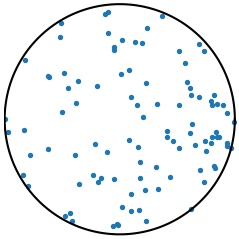
\includegraphics[width=0.13\textwidth]{ch-lcnet/images/Dataset/syn_test/MERL_directions}}
    \quad
    \raisebox{1.3\height}{\makebox[0.07\textwidth]{\makecell{\footnotesize Around \\ \footnotesize Equator}}}
    \makebox[0.13\textwidth]{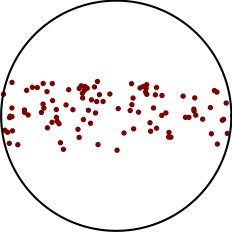
\includegraphics[width=0.13\textwidth]{ch-lcnet/images/Results/synth/equator_light.jpg}} 
    \quad
    \raisebox{1.3\height}{\makebox[0.07\textwidth]{\makecell{\footnotesize Around \\ \footnotesize Poles}}}
    \makebox[0.13\textwidth]{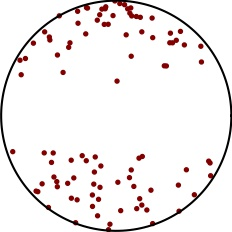
\includegraphics[width=0.13\textwidth]{ch-lcnet/images/Results/synth/polar_light.jpg}}
    \\
    \makebox[0.48\textwidth]{\small (a) Three different lighting distributions} 
    \\ \vspace{0.5em}
    \tdplotsetmaincoords{70}{100}
\pgfmathsetmacro{\rvec}{1}
\pgfmathsetmacro{\thetavec}{52}
\pgfmathsetmacro{\phivec}{45}
\pgfmathsetmacro{\dev}{18}
\pgfmathsetmacro{\tha}{\thetavec-\dev}
\pgfmathsetmacro{\thb}{\thetavec+\dev}
\pgfmathsetmacro{\phia}{\phivec-\dev}
\pgfmathsetmacro{\phib}{\phivec+\dev}

\begin{tikzpicture}[scale=2.2,tdplot_main_coords]
    \coordinate (O) at (0,0,0); %
    \draw[->] (0,0,0) -- (1,0,0) node[below=0.5ex,left=-0.4ex]{$z$};
    \draw[->] (0,0,0) -- (0,1,0) node[right=-0.4ex]{$x$};
    \draw[->] (0,0,0) -- (0,0,1) node[above=-0.4ex]{$y$};
    \draw[dashed,color=gray] (0,0,0) -- (0,0,-1);
    \draw[dashed,color=gray] (0,0,0) -- (0,-1,0);
    \tdplotdrawarc[semithick,dashed,color=gray]{(O)}{1}{-90}{90}{}{}
    \tdplotsetthetaplanecoords{90}
    \tdplotdrawarc[semithick,dashed,color=gray,tdplot_rotated_coords]{(0,0,0)}{1}{0}{360}{}{}

    \tdplotsetcoord{P}{\rvec}{\thetavec}{\phivec} %
    \draw[thick,-stealth,color=black] (O) -- (P) node[below=0.2ex,right=-1.0ex] {$P$};

    \tdplotsetcoord{Pa}{\rvec}{\tha}{\phia}
    \tdplotsetcoord{Pb}{\rvec}{\tha}{\phib}
    \tdplotsetcoord{Pc}{\rvec}{\thb}{\phia}
    \tdplotsetcoord{Pd}{\rvec}{\thb}{\phib}
    \tdplotsetcoord{Pf}{\rvec}{\tha}{\phivec}

    \draw[color=black] (O) -- (Pa) node[above=0.2ex,left=-0.7ex] {\color{black!90}\scriptsize $A$};
    \draw[color=black] (O) -- (Pb) node[above,right=-0.3ex] {\color{black!90}\scriptsize $B$};
    \draw[color=black] (O) -- (Pc) node[below=1.2ex,left=-0.9ex] {\color{black!90}\scriptsize $C$};
    \draw[color=black] (O) -- (Pd) node[below=0.2ex,right=-0.3ex] {\color{black!90}\scriptsize $D$};
    \draw[color=blue,dashed] (O) -- (Pf) node[above left] {};

    \draw[semithick,color=red] (Pa) to  (Pb) node[below left] {};
    \draw[semithick,color=red] (Pd) to  (Pc) node[below left] {};

    \tdplotsetthetaplanecoords{\phivec}
    \tdplotdrawarc[thick,color=blue,opacity=0.8,tdplot_rotated_coords]{(0,0,0)}{0.7}{\tha}{\thetavec}{above=0.7ex,right=-0.7ex}{\small $\delta$}
    \tdplotsetthetaplanecoords{\phia}
    \tdplotdrawarc[semithick,color=red,tdplot_rotated_coords]{(0,0,0)}{\rvec}{\tha}{\thb}{anchor=south west}{}
    \tdplotdrawarc[dashed,tdplot_rotated_coords]{(0,0,0)}{\rvec}{0}{\tha}{anchor=south west}{}
    \tdplotdrawarc[dashed,tdplot_rotated_coords]{(0,0,0)}{\rvec}{\thb}{180}{anchor=south west}{}
    \tdplotsetthetaplanecoords{\phib}
    \tdplotdrawarc[semithick,color=red,tdplot_rotated_coords]{(0,0,0)}{\rvec}{\tha}{\thb}{anchor=south west}{}
    \tdplotdrawarc[dashed,tdplot_rotated_coords]{(0,0,0)}{\rvec}{0}{\tha}{anchor=south west}{}
    \tdplotdrawarc[dashed,tdplot_rotated_coords]{(0,0,0)}{\rvec}{\thb}{180}{anchor=south west}{}

\end{tikzpicture}

    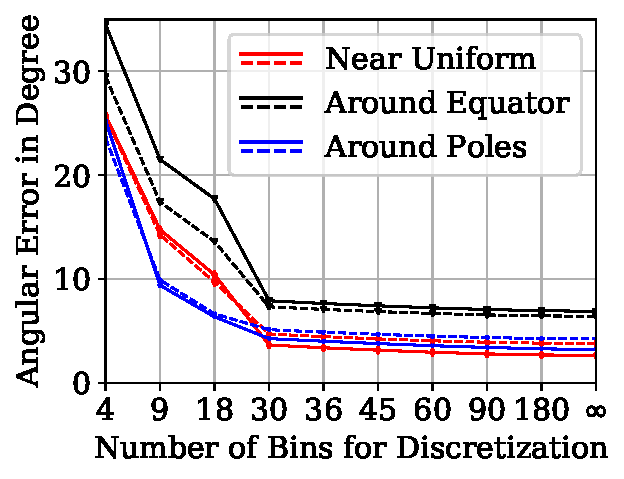
\includegraphics[width=0.40\textwidth]{ch-lcnet/images/Results/Discretization/Discretization_Error_sphere_uniform_error_combine.pdf}
    \\
    \vspace{-0.6em}  
    \makebox[0.30\textwidth]{\small (b)}
    \makebox[0.37\textwidth]{\small (c)}

    \caption[Results of LCNet under different light direction space discretization levels]{(a) Three different lighting distributions. (b) Light directions $A$, $B$, $C$, and $D$ have the maximum deviation angles with the actual light direction $P$ after discretization. (c) Normal estimation error of PS-FCN on \emphobject{Sphere} (solid lines) and \emphobject{Bunny} (dashed lines) under different light direction space discretization levels ($\infty$ indicates no discretization).} \label{fig:discretization}
\end{figure}

\paragraph{Effectiveness of LCNet}
We first investigated the effect of object mask input and local-global feature fusion.
\Tref{tab:quant_light_synth} shows that taking the object mask as input and adopting the proposed local-global feature fusion strategy can effectively improve the lighting estimation results.
This might be explained by that object mask helps the network distinguish the shadow region from the non-object region, while the proposed local-global feature fusion strategy can effectively make use of information from multiple observations. 

\begin{table}[tbp] \centering
    \caption[Lighting estimation results of LCNet on \syntestMERL dataset]{Lighting estimation results (MAE in degree for light direction and relative error for intensity) on \syntestMERL dataset. The results are averaged over samples rendered with $100$ BRDFs. (Value the lower the better)}
    \resizebox{0.9\textwidth}{!}{
    \large
\begin{tabular}{l|*{2}{c}|*{2}{c}|*{2}{c}|*{2}{c}}
    \toprule
    & \multicolumn{2}{c}{{\sc Sphere}} & \multicolumn{2}{c}{{\sc Bunny}} & \multicolumn{2}{c}{{\sc Dragon}} & \multicolumn{2}{c}{{\sc Armadillo}}\\
    Model  & Direction    & Intensity  & Direction    & Intensity  & Direction    & Intensity  & Direction    & Intensity  \\
    \midrule
    LCNet                     & \B{3.47} & \B{0.082} & \B{5.38}  & \B{0.089} & \B{7.85} & \B{0.096} & \B{7.50}  & \B{0.103}\\ %
    LCNet$_{\text{w/o mask}}$ & 5.46     & 0.104     & 8.85      & 0.144 & 11.81 & 0.176 & 13.02 & 0.166\\ %
    LCNet$_{\text{local}}$    & 6.87     & 0.198     & 9.98      & 0.255 & 10.58 & 0.264 & 9.50 & 0.266 \\ %
    \bottomrule
\end{tabular}
}
 \label{tab:quant_light_synth}
\end{table}

\begin{table}[tbp] \centering
    \caption[Results on \emphobject{Sphere} and \emphobject{Bunny} under different lighting distributions]{Results of LCNet and \LCNetreg on \emphobject{Sphere} and \emphobject{Bunny} rendered under different lighting distributions.} \label{tab:quant_light_synth_regression}
    \resizebox{\textwidth}{!}{
    \Huge
\begin{tabular}{l|*{4}{c}|*{4}{c}|*{4}{c}}
    \toprule
    & \multicolumn{4}{c}{Near Uniform} & \multicolumn{4}{c}{Around Equator} & \multicolumn{4}{c}{Around Poles} \\
    & \multicolumn{2}{c}{{\sc Sphere}} & \multicolumn{2}{c|}{{\sc Bunny}} & \multicolumn{2}{c}{{\sc Sphere}} & \multicolumn{2}{c}{{\sc Bunny}} & \multicolumn{2}{c}{{\sc Sphere}} & \multicolumn{2}{c}{{\sc Bunny}}\\
    Model  & Direction    & Intensity   & Direction    & Intensity  & Direction    & Intensity  & Direction    & Intensity  & Direction    & Intensity  & Direction    & Intensity  \\
    \midrule
    LCNet                 & \B{3.47} & \B{0.082} & \B{5.38}  & \B{0.089} & \B{3.32} & \B{0.079} & \B{5.33} & \B{0.077} & \B{4.82} & \B{0.088} & \B{6.34} & \B{0.095} \\
    \LCNetreg  & 4.10     & 0.104     & 5.46  & 0.094  & 3.72 & 0.091 & 5.85 & 0.092 & 5.57 & 0.104 & 7.47 & 0.102 \\ 
    \bottomrule
\end{tabular}
}
 
\end{table}

We then compared LCNet with a regression based baseline, denoted as \LCNetreg, to validate the effectiveness of the classification based model.
\LCNetreg shares the same architecture with LCNet, except that LCNet$_{\text{reg}}$ estimates a 3-vector for light direction and a scalar value for light intensity, rather than the softmax probability vectors.
 Given $q$ images, the loss function for the lighting regression is
 \begin{align}
     \label{eq:loss_reg}
     \mathcal{L}_{\text{Reg}} & = \lambda_{l} \frac{1}{q} \sum_{i}^q (1 - \boldsymbol{l}_{i}^\top \tilde{\boldsymbol{l}}_{i} )+ \lambda_{e} \frac{1}{q} \sum_{i}^q (e_{i} - \tilde{e}_{i} )^2,
 \end{align}
 where $\lambda_{l}$ and $\lambda_{e}$ are the weighting factors for the loss terms, $\boldsymbol{l}_{i}$ ($e_{i}$) and $\tilde{\boldsymbol{l}}_{i}$ ($\tilde{e}_{i}$) denote the predicted light direction (intensity) and the ground truth, respectively, for image $i$. During training, $\lambda_{l}$ and $\lambda_{e}$ are set to 1 (we found that using other weighting factors produce similar results).


Specifically, we tested LCNet and \LCNetreg on three different lighting distributions illustrated in \fref{fig:discretization}~(a). The results are shown in \Tref{tab:quant_light_synth_regression}. The proposed classification based LCNet consistently outperforms \LCNetreg on both light direction and intensity estimation. This echoes our hypothesis that classifying a light direction to a certain range is easier than regressing an exact value. Thus, solving the classification problem reduces the learning difficulty and improves the performance.
It can also be seen that both methods perform better on \textit{Around Equator} and worse on \textit{Around Poles}.
This suggests that lightings around the poles are more difficult to estimate due to their extremely directions, independent of the lighting space discretization.

\begin{figure}[htbp] \centering
    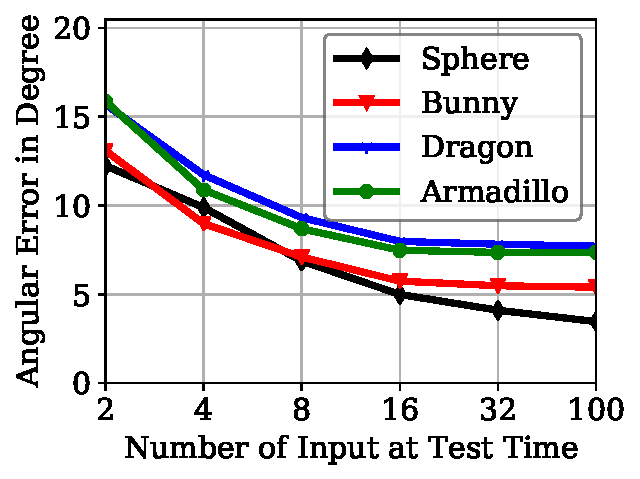
\includegraphics[width=0.46\textwidth]{ch-lcnet/images/Results/synth/SDPS-Net_img_sense_direction_img_num_sensitivity.pdf}
    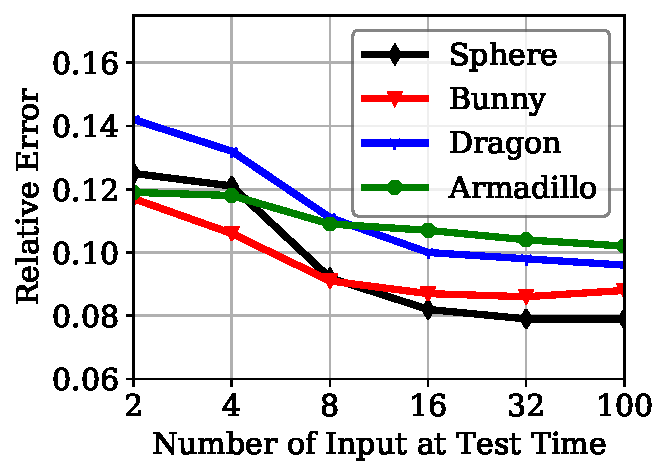
\includegraphics[width=0.48\textwidth]{ch-lcnet/images/Results/synth/SDPS-Net_img_sense_intensity_img_num_sensitivity.pdf}
    \\ \vspace{-0.5em}
    \makebox[0.46\textwidth]{\footnotesize (a) Light direction estimation}
    \makebox[0.48\textwidth]{\footnotesize (b) Light intensity estimation}\\
    \caption[Results of LCNet on \syntestMERL dataset with varying image numbers]{Lighting estimation results of LCNet on \syntestMERL dataset with varying input image numbers.} \label{fig:img_num_syn}
\end{figure}

\Fref{fig:img_num_syn} shows that the performance of LCNet increases with the number of input images. This is expected, since more useful information can be used to infer lightings with more input images.


\newcommand{\PSFCNdag}{PS-FCN$^\dag$\xspace}

\paragraph{Integration with PS-FCN for normal estimation}
For uncalibrated photometric stereo, we train a variant of PS-FCN, denoted as \PSFCNdag, using the lighting estimated by LCNet. 
Note that the weights of LCNet was fixed during the training of \PSFCNdag, as we found that end-to-end fine-tuning did not improve the performance.  
Experiments with IDs C1 \& C2 in \Tref{tab:quant_normal_syn} show that after training with the discretized lighting estimated by LCNet, \PSFCNdag performs better than PS-FCN given possibly noisy lightings at test time. Besides, experiments with IDs C2 \& C3 show that \PSFCNdag coupled with the classification based LCNet consistently outperforms that with the regression based \LCNetreg. 

\begin{table}[tbp] \centering
    \caption[Normal estimation results on \syntestMERL dataset]{Normal estimation results on \syntestMERL dataset. \PSFCNdag was trained given lightings estimated by LCNet or \LCNetreg.} %
    \resizebox{0.7\textwidth}{!}{
\Huge
\begin{tabular}{cl|c|*{1}{c}*{1}{c}*{1}{c}*{1}{c}}
\toprule
ID & Model  & \# Param & {\sc Sphere} & {\sc Bunny} & {\sc Dragon} & {\sc Armad.}\\
\midrule
C0 & PS-FCN                      & 2.2 M & 2.66   & 3.80 & 4.83 & 5.24\\ %
\midrule 
C1 & LCNet + PS-FCN                      & 6.6 M & 3.19  & 4.67 & 6.92 & 7.70\\ %
\rowcolor{gray!30}
C2 & LCNet + PS-FCN$^\dag$& 6.6 M        & \B{2.71} & \B{4.09} & \B{6.41} & \B{7.09}\\%vis7 Mid
C3 & LCNet$_{\text{reg}}$ + PS-FCN$^\dag$ & 6.6 M & 3.22  & 4.99 & 6.63 & 7.54\\ %
\midrule
C4 & UPS-FCN$_{\text{deep+mask}}$   & 6.1 M & 3.65 & 6.41 & 9.68 & 11.26   \\ %
C5 & UPS-FCN     & 2.2 M & 7.44 & 12.34 & 14.44 & 15.93 \\ %
\bottomrule
\end{tabular}
}
 \label{tab:quant_normal_syn}
\end{table}


\paragraph{Comparison with single-stage deep uncalibrated models}
To validate the effectiveness of the proposed two-stage approach, we compared our method with two different single-stage baseline models.
We first train a variant of PS-FCN, denoted as UPS-FCN, without taking the light direction as input during training and testing.
We then increased the model capacity of UPS-FCN by training a deeper network, denoted as UPS-FCN$_{\text{deep+mask}}$, that takes both the images and object mask as input (see \fref{fig:upsfcn_model_variants}). 

\begin{figure}[tbp] \centering
    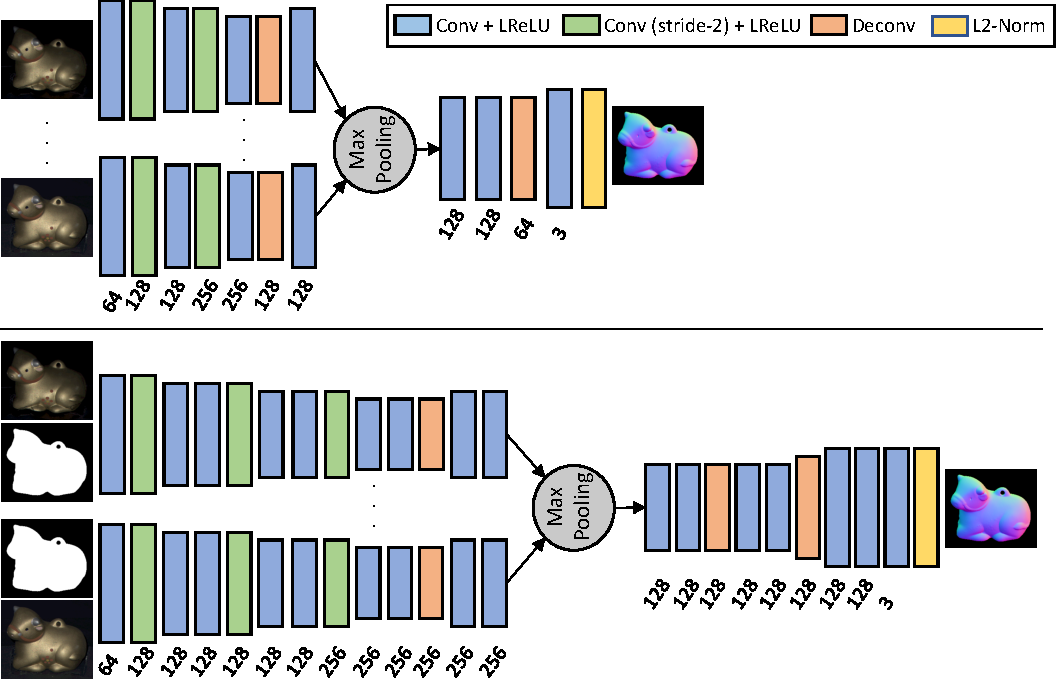
\includegraphics[width=\textwidth]{ch-lcnet/images/Method/UPS-FCN_Variants}
    \caption[Network architectures of UPS-FCN and UPS-FCN$_{\text{deep+mask}}$.]{Network architectures of UPS-FCN (top) and UPS-FCN$_{\text{deep+mask}}$ (bottom).} \label{fig:upsfcn_model_variants}
\end{figure}

Experiments with IDs C4 \& C5 in \Tref{tab:quant_normal_syn} show that utilizing a deeper network and taking the object mask as input can improve the performance of single-stage model.
However, experiments with IDs C2 \& C4 show that the proposed method significantly outperforms the single-stage model, when the input as well as the number of parameters are comparable.
This result indicates that simply increasing the depth of the network cannot produce optimal results. 



\section{Analyzing What is Learned in LCNet}
\label{sec:LCNet_analysis}
\Sref{sub:eval_lcnet} shows that the proposed LCNet can predict accurate lightings for different testing objects. Also, given the lightings estimated by LCNet, the calibrated method PS-FCN significantly outperforms the single-stage uncalibrated method UPS-FCN.
However, what specifically inside the LCNet contributes to its success remains a mystery.

In this section, we discuss the inherent ambiguity in uncalibrated photometric stereo of Lambertian surfaces, the fact that it can be resolved for non-Lambertian surfaces, and the features learned by LCNet to resolve such ambiguity.

\newcommand{\numpixels}{\ensuremath{P}}
\newcommand{\pixelindex}{\ensuremath{p}}
\newcommand{\numlightings}{\ensuremath{F}}
\newcommand{\lightingindex}{\ensuremath{f}}
\subsection{Lambertian Surfaces and the \gbr Ambiguity}
When ignoring shadows (\ie, attached and cast shadows) and inter-reflections, the image formation of a Lambertian surface with $\numpixels$ pixels captured under $\numlightings$ lightings can be written as
\begin{equation}
    \V{M} = \V{N}^\top \V{L},
\end{equation}
where \hbox{$\V{M} \in \mathbb{R}^{\numpixels \times \numlightings}$} is the measurement matrix. 
\hbox{$\V{N} \in \mathbb{R}^{3\times \numpixels}$} is the surface normal matrix whose columns are albedo scaled normals \hbox{$\V{N}_{:,\pixelindex}=\rho_\pixelindex\vn_\pixelindex$}, where $\rho_\pixelindex$ and $\vn_\pixelindex$ are the albedo and unit-length surface normal of pixel $\pixelindex$.
\hbox{$\V{L} \in \mathbb{R}^{3\times \numlightings}$} is the lighting matrix whose columns are intensity scaled light directions $\V{L}_{:,f} = e_f\vl_f$, where $e_f$ and $\vl_f$ are the light intensity and unit-length light direction of image~$f$.

\begin{figure}[htbp] \centering
	    \makebox[0.115\textwidth]{\footnotesize (a) Normal}
    \makebox[0.115\textwidth]{\footnotesize (b) Albedo} 
   \makebox[0.1150\textwidth]{\footnotesize (c) Lighting}
    \makebox[0.002\textwidth]{} 
    \makebox[0.355\textwidth]{\footnotesize (d) Sample Images}
    \makebox[0.115\textwidth]{\footnotesize (e) PF14}
    \makebox[0.115\textwidth]{\footnotesize (f) LCNet}
    \\
     \makebox[0.115\textwidth]{
\includegraphics[width=0.115\textwidth]{ch-gcnet/images/Intro/GBR/origin_sphere/1_1_5.png}}
     \makebox[0.115\textwidth]{
\includegraphics[width=0.115\textwidth]{ch-gcnet/images/Intro/GBR/origin_sphere/1_1_4.png}}
      \makebox[0.115\textwidth]{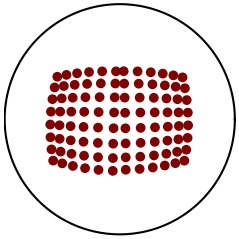
\includegraphics[width=0.115\textwidth]{ch-gcnet/images/Intro/GBR/origin_sphere/ballPNG_gt_lighting.jpg}
     \hspace{-0.5em} \raisebox{0.1em}{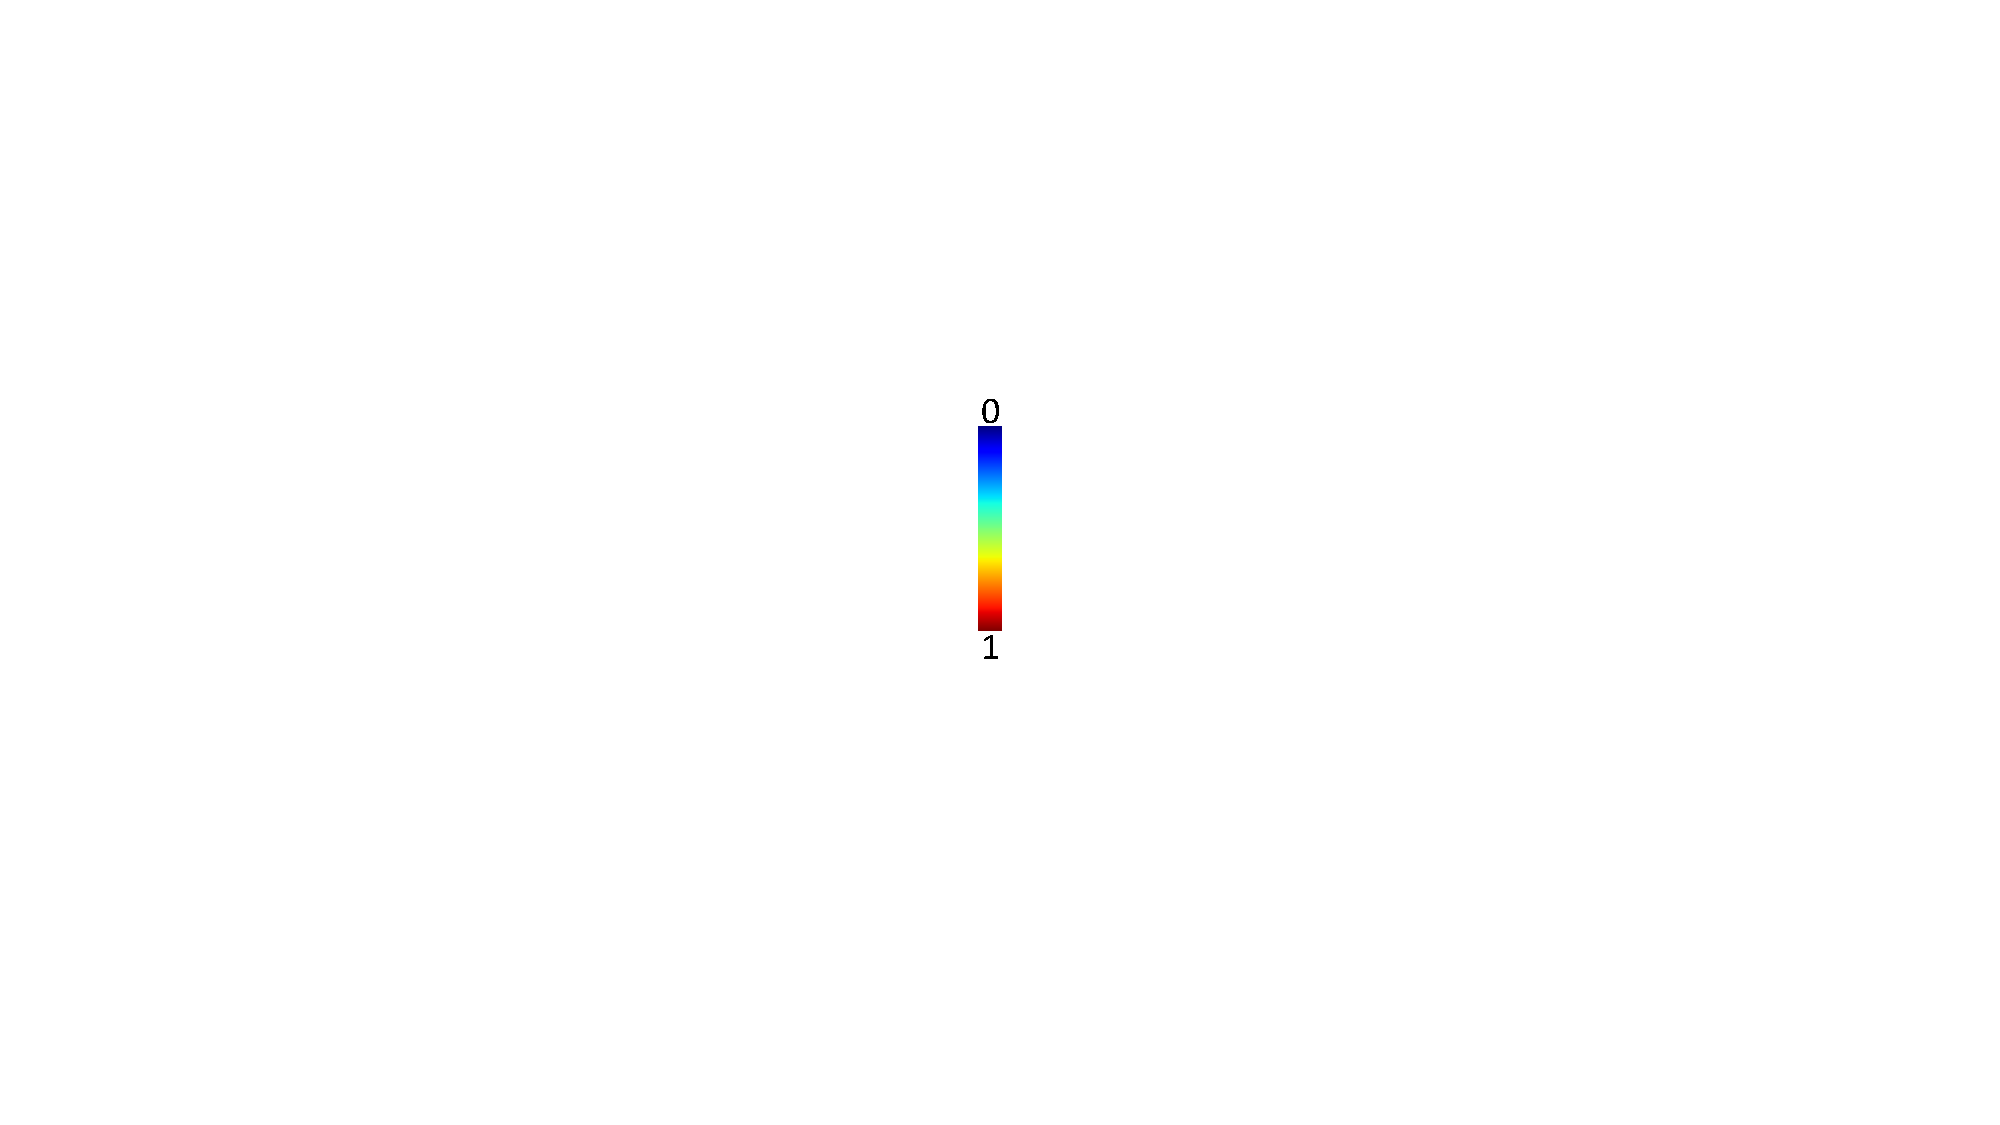
\includegraphics[height=0.10\textwidth]{ch-gcnet/images/Intro/colorbar_jet.pdf}}}
     \makebox[0.115\textwidth]{\includegraphics[width=0.115\textwidth]{ch-gcnet/images/Intro/GBR/origin_sphere/1_1_0.png}}
     \makebox[0.115\textwidth]{\includegraphics[width=0.115\textwidth]{ch-gcnet/images/Intro/GBR/origin_sphere/1_1_1.png}}
     \makebox[0.115\textwidth]{\includegraphics[width=0.115\textwidth]{ch-gcnet/images/Intro/GBR/origin_sphere/1_1_3.png}}
     \makebox[0.115\textwidth]{
\includegraphics[width=0.115\textwidth]{ch-gcnet/images/Intro/GBR/PF14_ballPNG.jpg}}
     \makebox[0.115\textwidth]{\includegraphics[width=0.115\textwidth]{ch-gcnet/images/Intro/GBR/origin_sphere/ballPNG_est_lighting.jpg}}
     \\
     \makebox[0.115\textwidth]{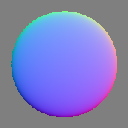
\includegraphics[width=0.115\textwidth]{ch-gcnet/images/Intro/GBR/flatten_sphere/1_1_5.png}}
     \makebox[0.115\textwidth]{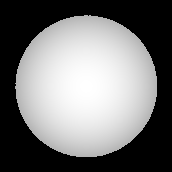
\includegraphics[width=0.115\textwidth]{ch-gcnet/images/Intro/GBR/flatten_sphere/albedo_ballPNG.png}}
      \makebox[0.115\textwidth]{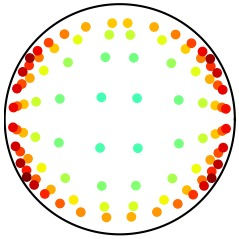
\includegraphics[width=0.115\textwidth]{ch-gcnet/images/Intro/GBR/flatten_sphere/ballPNG_gt_lighting.jpg}
     \hspace{-0.5em} \raisebox{0.1em}{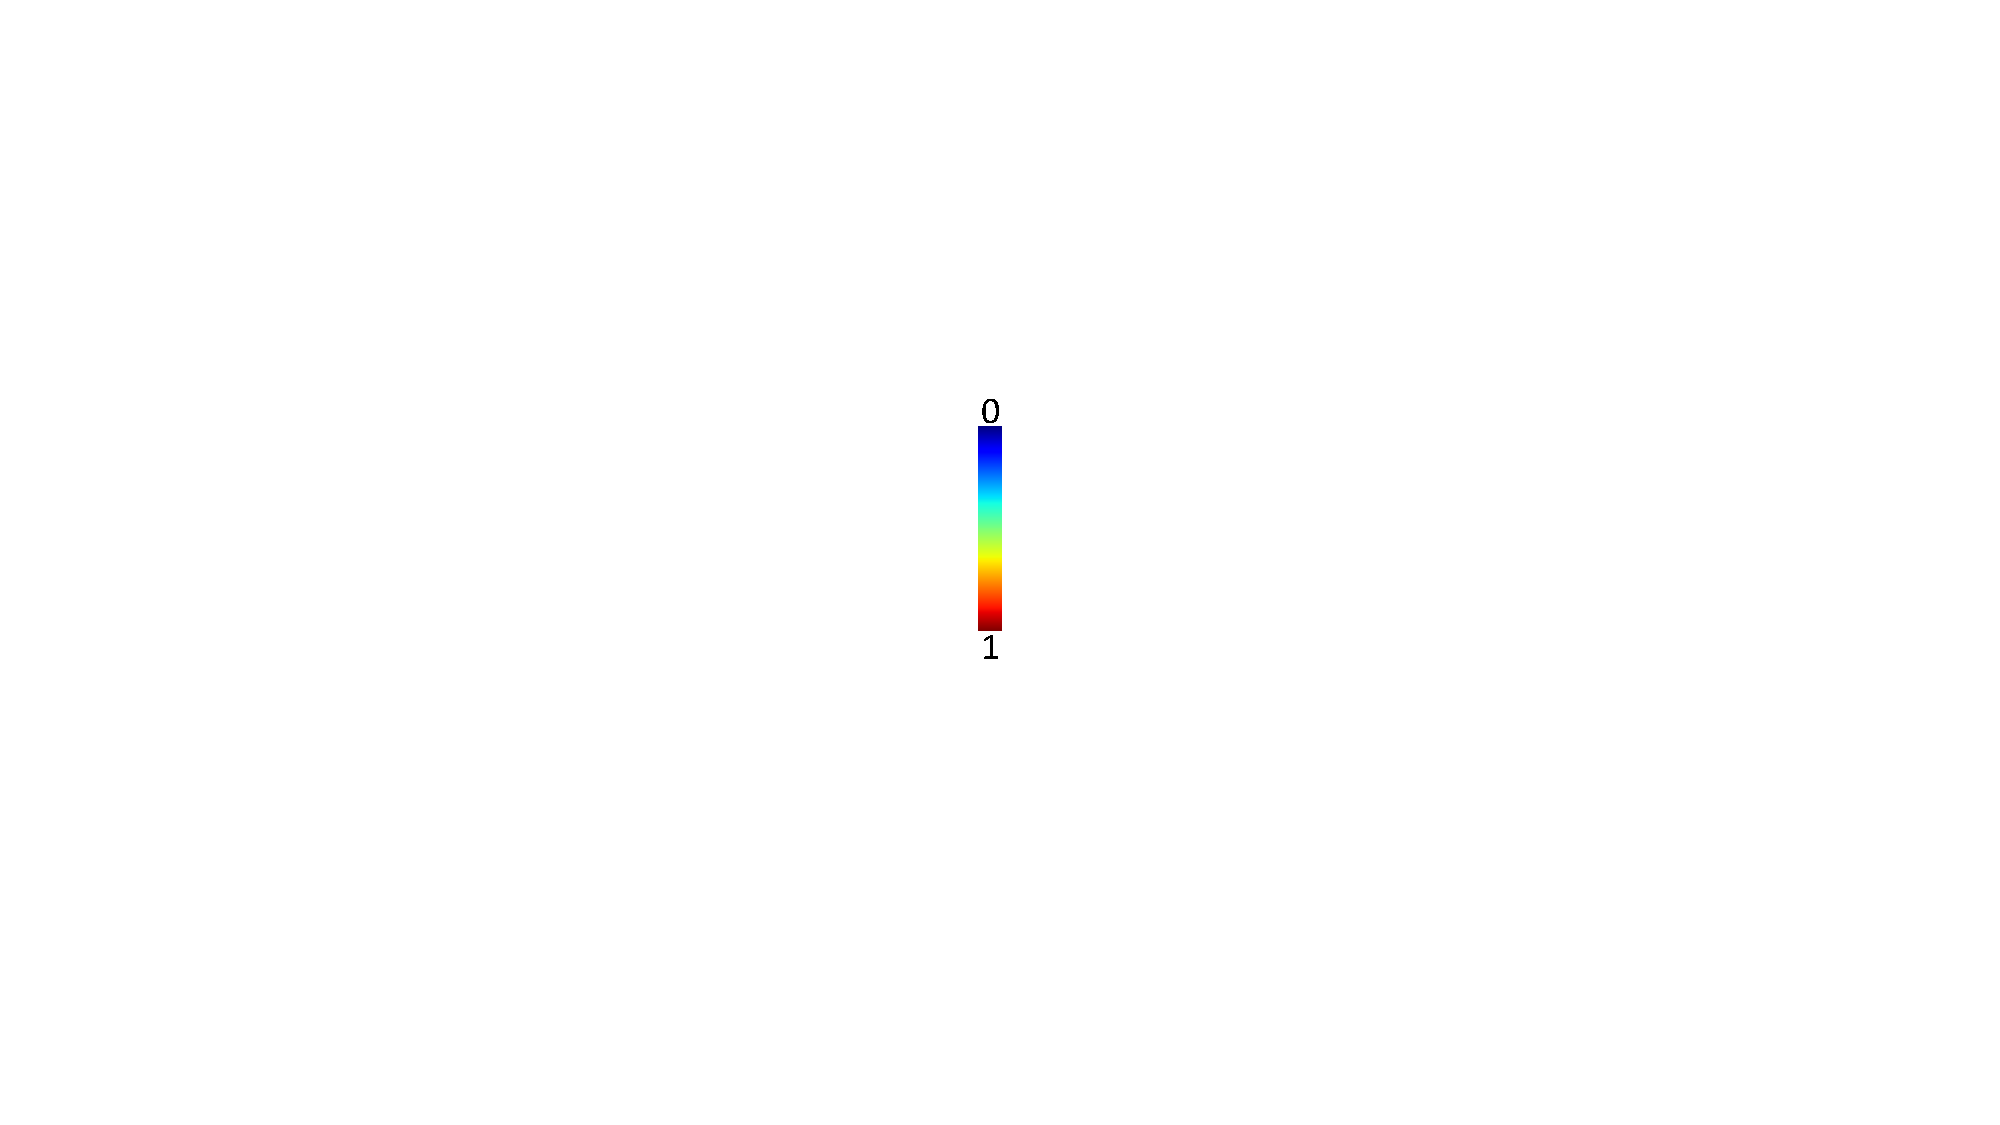
\includegraphics[height=0.10\textwidth]{ch-gcnet/images/Intro/colorbar_jet.pdf}}}
     \makebox[0.115\textwidth]{\includegraphics[width=0.115\textwidth]{ch-gcnet/images/Intro/GBR/flatten_sphere/1_1_0.png}}
     \makebox[0.115\textwidth]{\includegraphics[width=0.115\textwidth]{ch-gcnet/images/Intro/GBR/flatten_sphere/1_1_1.png}}
     \makebox[0.115\textwidth]{\includegraphics[width=0.115\textwidth]{ch-gcnet/images/Intro/GBR/flatten_sphere/1_1_3.png}}
     \makebox[0.115\textwidth]{
\includegraphics[width=0.115\textwidth]{ch-gcnet/images/Intro/GBR/PF14_ballPNG.jpg}}
     \makebox[0.115\textwidth]{\includegraphics[width=0.115\textwidth]{ch-gcnet/images/Intro/GBR/flatten_sphere/ballPNG_est_lighting.jpg}}
    \\
    \makebox[0.115\textwidth]{
\includegraphics[width=0.115\textwidth]{ch-gcnet/images/Intro/GBR/slanted_sphere/1_1_5.png}}
    \makebox[0.115\textwidth]{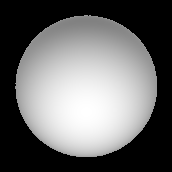
\includegraphics[width=0.115\textwidth]{ch-gcnet/images/Intro/GBR/slanted_sphere/albedo_ballPNG.png}}
     \makebox[0.115\textwidth]{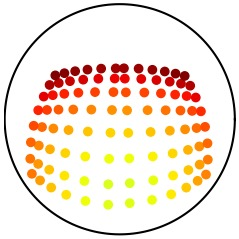
\includegraphics[width=0.115\textwidth]{ch-gcnet/images/Intro/GBR/slanted_sphere/ballPNG_gt_lighting.jpg}
     \hspace{-0.5em} \raisebox{0.1em}{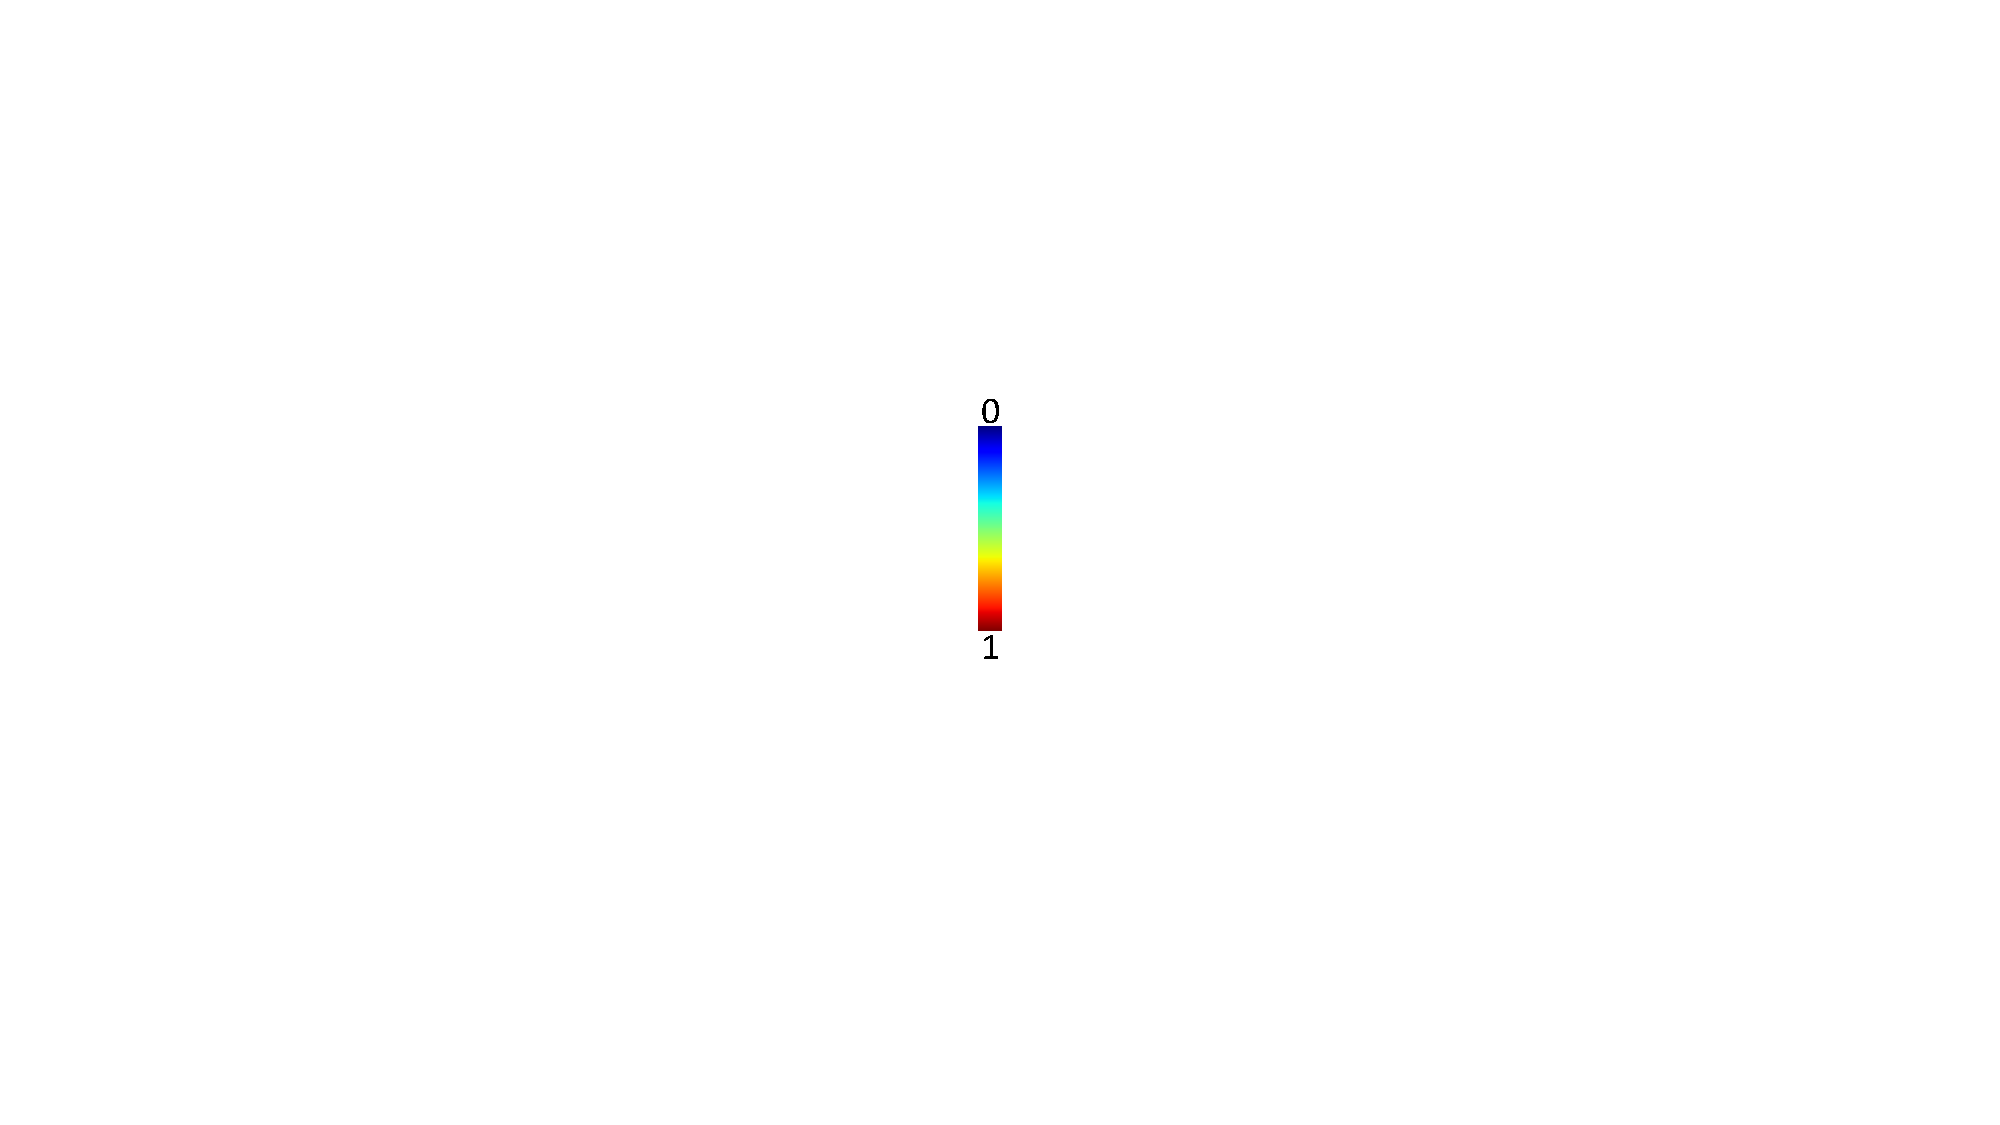
\includegraphics[height=0.10\textwidth]{ch-gcnet/images/Intro/colorbar_jet.pdf}}}
    \makebox[0.115\textwidth]{\includegraphics[width=0.115\textwidth]{ch-gcnet/images/Intro/GBR/slanted_sphere/1_1_0.png}}
    \makebox[0.115\textwidth]{\includegraphics[width=0.115\textwidth]{ch-gcnet/images/Intro/GBR/slanted_sphere/1_1_1.png}}
    \makebox[0.115\textwidth]{\includegraphics[width=0.115\textwidth]{ch-gcnet/images/Intro/GBR/slanted_sphere/1_1_3.png}}
    \makebox[0.115\textwidth]{
\includegraphics[width=0.115\textwidth]{ch-gcnet/images/Intro/GBR/PF14_ballPNG.jpg}}
    \makebox[0.115\textwidth]{\includegraphics[width=0.115\textwidth]{ch-gcnet/images/Intro/GBR/flatten_sphere/ballPNG_est_lighting.jpg}}
    \\

    \caption[Results of PF14 and LCNet on shapes under different GBR transformation]{Row~1 is the true shape of a \emphobject{Sphere}, while rows~2 and~3 are shapes under two different GBR transformations. In column~(c), the points' positions and colors indicate light direction and relative intensity, respectively. Columns (e) and (f) show the lightings estimated by PF14~\cite{papad14closed} and LCNet.}\label{fig:gbr}
\end{figure}
    
By matrix factorization and applying the surface integrability constraint, $\V{N}$ and $\V{L}$ can be recovered up to an unknown $3$-parameter GBR transformation $\V{G}$~\cite{belhumeur1999bas} such that \hbox{$\V{M} = (\V{G}^{-\top}\V{N})^\top (\V{G}\V{L})$}. This GBR ambiguity indicates that there are infinitely many combinations of albedo $\rho$, normal $\vn$, light direction $\vl$, and light intensity~$e$ that produce the same appearance $\V{M}$ (see~\fref{fig:gbr}~(a)-(d)):
\begin{align}
    \hat{\rho} \!=\! \rho|\V{G}^{-\top}\vn|,\,\,
    \hat{\vn} \!=\! \frac{\V{G}^{-\top}\vn}{|\V{G}^{-\top}\vn|},\,\,
    \hat{\vl} \!=\! \frac{\V{G}\vl}{|\V{G}\vl|},\,\,
    \hat{e} \!=\! e |\V{G} \vl|.
\end{align}

Although the surface's appearance remains the same after GBR transformation (\ie, \hbox{$\hat{\rho} \hat{\vn}^{\!\top} \hat{\vl}  \hat{e} \!=\! \rho \vn^\top \vl e$}, see \fref{fig:gbr}~(d)), a surface point's albedo will be scaled by \hbox{$|\V{G}^{-\top} \vn|$}. As a result, the albedo of an object will change gradually and become spatially-varying. 
Because this
kind of spatially-varying albedo distribution resulting %
from \gbr transformations rarely occurs on real world objects, some previous methods make explicit assumptions on the albedo distribution (\eg, constant albedo~\cite{belhumeur1999bas,papad14closed} or low entropy~\cite{alldrin2007r}) to resolve the ambiguity.

PF14~\cite{papad14closed}, a state-of-the-art non-learning uncalibrated method~\cite{shi2019benchmark}, detects Lambertian diffuse reflectance maxima (\ie, image points satisfying $\vn^\top\vl=1$) to estimate $\V{G}$'s $3$ parameters. %
We will later use it as a non-learning benchmark in our comparative experiments.


\subsection{LCNet and the GBR Ambiguity}
\Fref{fig:gbr}~(e)-(f) compare the results of LCNet and PF14 on surfaces that differ by GBR transformations. 
Since the input images are the same in all cases, LCNet estimates the same lightings in all cases, namely the most likely lightings for the input images. The same also applies to PF14.
Although LCNet's result does not exactly equal the lightings for uniform albedo, we note that it learned from the training data that GBR-transformed surfaces are unlikely.

\begin{table}[t] \centering
    \caption[Results of PF14 and LCNet on a \emphobject{Sphere} rendered with different BRDFs]{Light direction estimation results of PF14~\cite{papad14closed} and LCNet on a \emphobject{Sphere} rendered with different BRDF types. Non-Lambertian BRDFs are taken from the MERL dataset~\cite{matusik2003merl}.} \label{tab:res_sphere_brdfs}
    \resizebox{0.9\linewidth}{!}{%
     \begin{tabular}{l*{5}{c}c}%
        \toprule
         & 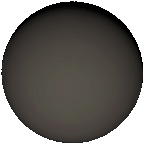
\includegraphics[width=0.15\textwidth]{ch-gcnet/images/Intro/Compare_PF14/Lambertian}
         & 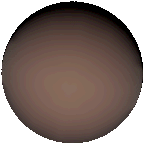
\includegraphics[width=0.15\textwidth]{ch-gcnet/images/Intro/Compare_PF14/beige-fabric}
         & 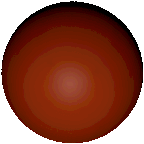
\includegraphics[width=0.15\textwidth]{ch-gcnet/images/Intro/Compare_PF14/red-plastic}
         & 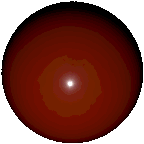
\includegraphics[width=0.15\textwidth]{ch-gcnet/images/Intro/Compare_PF14/red-phenolic}
         & 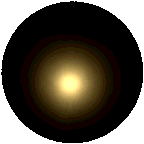
\includegraphics[width=0.15\textwidth]{ch-gcnet/images/Intro/Compare_PF14/gold-metallic-paint}
         \vspace{-0.3em}
         \\
         Model  & Lambertian & Fabric & Plastic & Phenolic & Metallic  & Avg.\\
        \midrule
         PF14 & 7.19 & 14.26 & 28.04 & 47.96 & 31.12 & 25.7 \\
         LCNet & \B{5.38} & \B{4.07} & \B{3.08} & \B{3.05} & \B{4.09} & \B{3.93} \\ 
        \bottomrule%
    \end{tabular}%
}%


\end{table}

Although uncalibrated photometric stereo has an intrinsic GBR ambiguity for Lambertian surfaces, it was shown that GBR transformations do not preserve specularities~\cite{belhumeur1999bas,georghiades2003incorporating,drbohlav2005can}. Hence, specularities are helpful for ambiguity-free lighting estimation.
However, traditional methods often treat non-Lambertian observations as outliers, and thus fail to %
make full use of specularities for disambiguation~\cite{papad14closed}.
In contrast, learning-based methods can learn the relation between specular highlights and light directions through end-to-end learning.
As shown in \Tref{tab:res_sphere_brdfs}, LCNet achieves good results for non-Lambertian surfaces while PF14 completely fails when non-Lambertian observations dominate.

\begin{figure}[htbp]\centering
	    \makebox[0.135\textwidth]{\footnotesize (a) Input}
    \makebox[0.420\textwidth]{\footnotesize (b) Highlight, Shadow, Shading}
    \makebox[0.420\textwidth]{\footnotesize (c) Extracted Local Features}
    \\
    \makebox[0.135\textwidth]{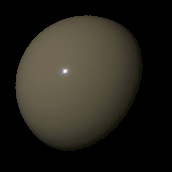
\includegraphics[width=0.135\textwidth]{ch-gcnet/images/Visualization/uniform_ints/048_gm.png}}
    \makebox[0.135\textwidth]{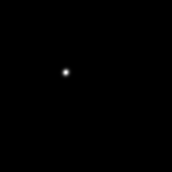
\includegraphics[width=0.135\textwidth]{ch-gcnet/images/Visualization/048_spec.png}}
    \makebox[0.135\textwidth]{
\includegraphics[width=0.135\textwidth]{ch-gcnet/images/Visualization/048_sd.png}}
    \makebox[0.135\textwidth]{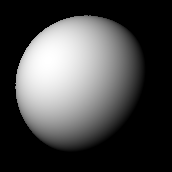
\includegraphics[width=0.135\textwidth]{ch-gcnet/images/Visualization/048_s.png}}
    \makebox[0.135\textwidth]{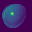
\includegraphics[width=0.135\textwidth]{ch-gcnet/images/Visualization/uniform_ints/ballPNG_000_236.png}}
    \makebox[0.135\textwidth]{
\includegraphics[width=0.135\textwidth]{ch-gcnet/images/Visualization/uniform_ints/ballPNG_000_238.png}}
    \makebox[0.135\textwidth]{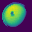
\includegraphics[width=0.135\textwidth]{ch-gcnet/images/Visualization/uniform_ints/ballPNG_000_254.png}}
    \\
    \makebox[0.135\textwidth]{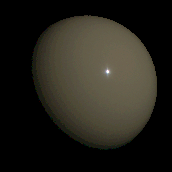
\includegraphics[width=0.135\textwidth]{ch-gcnet/images/Visualization/uniform_ints/096_gm.png}}
    \makebox[0.135\textwidth]{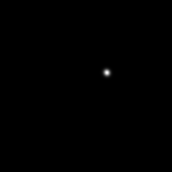
\includegraphics[width=0.135\textwidth]{ch-gcnet/images/Visualization/096_spec.png}}
    \makebox[0.135\textwidth]{\includegraphics[width=0.135\textwidth]{ch-gcnet/images/Visualization/096_sd.png}}
    \makebox[0.135\textwidth]{\includegraphics[width=0.135\textwidth]{ch-gcnet/images/Visualization/096_s.png}}
    \makebox[0.135\textwidth]{\includegraphics[width=0.135\textwidth]{ch-gcnet/images/Visualization/uniform_ints/ballPNG_011_236.png}}
    \makebox[0.135\textwidth]{\includegraphics[width=0.135\textwidth]{ch-gcnet/images/Visualization/uniform_ints/ballPNG_011_238.png}}
    \makebox[0.135\textwidth]{\includegraphics[width=0.135\textwidth]{ch-gcnet/images/Visualization/uniform_ints/ballPNG_011_254.png}}
    \\
    \makebox[0.135\textwidth]{\includegraphics[width=0.135\textwidth]{ch-gcnet/images/Visualization/uniform_ints/005_gm.png}}
    \makebox[0.135\textwidth]{\includegraphics[width=0.135\textwidth]{ch-gcnet/images/Visualization/005_spec.png}}
    \makebox[0.135\textwidth]{\includegraphics[width=0.135\textwidth]{ch-gcnet/images/Visualization/005_sd.png}}
    \makebox[0.135\textwidth]{\includegraphics[width=0.135\textwidth]{ch-gcnet/images/Visualization/005_s.png}}
    \makebox[0.135\textwidth]{\includegraphics[width=0.135\textwidth]{ch-gcnet/images/Visualization/uniform_ints/ballPNG_040_236.png}}
    \makebox[0.135\textwidth]{\includegraphics[width=0.135\textwidth]{ch-gcnet/images/Visualization/uniform_ints/ballPNG_040_238.png}}
    \makebox[0.135\textwidth]{\includegraphics[width=0.135\textwidth]{ch-gcnet/images/Visualization/uniform_ints/ballPNG_040_254.png}}
    \\
    \makebox[0.135\textwidth]{\includegraphics[width=0.135\textwidth]{ch-gcnet/images/Visualization/uniform_ints/041_gm.png}}
    \makebox[0.135\textwidth]{\includegraphics[width=0.135\textwidth]{ch-gcnet/images/Visualization/041_spec.png}}
    \makebox[0.135\textwidth]{\includegraphics[width=0.135\textwidth]{ch-gcnet/images/Visualization/041_sd.png}}
    \makebox[0.135\textwidth]{\includegraphics[width=0.135\textwidth]{ch-gcnet/images/Visualization/041_s.png}}
    \makebox[0.135\textwidth]{\includegraphics[width=0.135\textwidth]{ch-gcnet/images/Visualization/uniform_ints/ballPNG_084_236.png}}
    \makebox[0.135\textwidth]{\includegraphics[width=0.135\textwidth]{ch-gcnet/images/Visualization/uniform_ints/ballPNG_084_238.png}}
    \makebox[0.135\textwidth]{\includegraphics[width=0.135\textwidth]{ch-gcnet/images/Visualization/uniform_ints/ballPNG_084_254.png}}
    \\
    \makebox[0.135\textwidth]{\includegraphics[width=0.135\textwidth]{ch-gcnet/images/Visualization/uniform_ints/089_gm.png}} %
    \makebox[0.135\textwidth]{\includegraphics[width=0.135\textwidth]{ch-gcnet/images/Visualization/089_spec.png}} 
    \makebox[0.135\textwidth]{\includegraphics[width=0.135\textwidth]{ch-gcnet/images/Visualization/089_sd.png}}
    \makebox[0.135\textwidth]{\includegraphics[width=0.135\textwidth]{ch-gcnet/images/Visualization/089_s.png}}
    \makebox[0.135\textwidth]{\includegraphics[width=0.135\textwidth]{ch-gcnet/images/Visualization/uniform_ints/ballPNG_095_236.png}}
    \makebox[0.135\textwidth]{\includegraphics[width=0.135\textwidth]{ch-gcnet/images/Visualization/uniform_ints/ballPNG_095_238.png}}
    \makebox[0.135\textwidth]{\includegraphics[width=0.135\textwidth]{ch-gcnet/images/Visualization/uniform_ints/ballPNG_095_254.png}}
    \\
    \makebox[0.135\textwidth]{}
    \makebox[0.135\textwidth]{}
    \raisebox{2.0\height}{\makebox[0.25\textwidth]{\footnotesize Fused Features}}
    \makebox[0.025\textwidth]{\includegraphics[height=0.135\textwidth]{ch-gcnet/images/Visualization/colorbar.pdf}}
    \makebox[0.135\textwidth]{\includegraphics[width=0.135\textwidth]{ch-gcnet/images/Visualization/uniform_ints/ballPNG_236.png}}
    \makebox[0.135\textwidth]{\includegraphics[width=0.135\textwidth]{ch-gcnet/images/Visualization/uniform_ints/ballPNG_238.png}}
    \makebox[0.135\textwidth]{\includegraphics[width=0.135\textwidth]{ch-gcnet/images/Visualization/uniform_ints/ballPNG_254.png}}
    \\

    \caption[Feature visualization of \hbox{LCNet} on a non-Lambertian \emphobject{Sphere}]{Feature visualization of \hbox{LCNet} on a non-Lambertian \emphobject{Sphere}. \emph{Column~1:}~$5$ of the $96$ input images; \emph{Columns~2--4:}~Specular high\-light centers, attached shadows, and shading rendered from ground truth; \emph{Columns~5--7:}~$3$ of LCNet's $256$ features maps. The last row shows the global features produced by fusing local features with max-pooling. All features are normalized to $[0, 1]$ and color coded.} \label{fig:visualization}
\end{figure}

\subsection{Feature Analysis for LCNet}
To analyze the features learned by LCNet, we first visualize the learned local and global features. \Fref{fig:visualization} shows $3$ representative features selected from $256$ feature maps extracted by LCNet from images of a non-Lambertian \emphobject{Sphere} dataset. 
Comparing \fref{fig:visualization}'s Column 2 with Column 5, Column 3 with Column 6, and Column 4 with Column 7, we can see that some feature maps are highly correlated with attached shadows (regions where the angle $\measuredangle(\vn,\vl)\!\ge\! 90\degree$), shadings ($\vn^{\!\top}\vl$), and specular highlights (regions where $\vn$ is close to the half angle $\vh\!=\!\frac{\vl+\vv}{\abs{\vl+\vv}}$ of $\vl$ and viewing direction $\vv$). 
As discussed earlier in the related work (\Sref{sec:lcnet_relatedwork}), these provide strong clues for resolving the ambiguity. %

To further verify our observations, we did the following. We computed (a)~attached shadows, (b)~the ``specular components'' (with a bit of concept abuse, we denote $\vh^\top\vn$ as specular component), and (c)~shadings for the synthetic Blobby and Sculpture datasets from their ground-truth light directions and normals.
We then trained $4$ variants of the LCNet, taking (a), (b), (c), and (a) + (b) + (c), respectively, as input instead of regular images.
We compared these $4$ variant networks with LCNet (\ie, the network trained with Blobby and Sculpture images) on a synthetic test dataset introduced in \Sref{subsec:synthetic_data}. Similar to LCNet, the variant networks also took the object mask as input.
\Tref{tab:proxy} shows that the variant models achieve results comparable to or even better than the model trained on regular images. 

\begin{table}[t] \centering
    \caption[Results of LCNet trained with different inputs]{Light direction estimation results of LCNet trained with different inputs. Values indicate mean angular error in degree.} \label{tab:proxy}
    \centering
\resizebox{0.8\linewidth}{!}{%
     \begin{tabular}{l*{4}{c}c}%
        \toprule
         model input & \emphobject{Sphere} & \emphobject{Bunny}& \emphobject{Dragon} & \emphobject{Armadillo} \\ %
        \midrule
             images           & 3.03 & 4.88 & 6.30 & 6.37 \\ %
        \midrule
             (a) attached shadows  & 3.50 & 5.07 & 9.78 & 5.22 \\ %
             (b) specular component & 2.53 & 6.18 & 7.33 & 4.08 \\ %
             (c) shading    & \B{2.29} & \B{3.95} & \B{4.64} & \B{3.76} \\ %
             \midrule
             (a) + (b) + (c)  & 1.87 & 2.06 & 2.34 & 2.12 \\ %
        \bottomrule%
    \end{tabular}%
}%

\end{table}

We can see that shadings contribute more than attached shadows and specular components for lighting estimation. 
This is because shading information actually includes attached shadows (\ie, pixels with a zero value in the shading for synthetic data), and can be considered as an image of an object with uniform albedo (albedo equals to $1$). The uniform albedo constraint is a well-known clue for resolving the GBR ambiguity~\cite{belhumeur1999bas,papad14closed}.
In practice, attached shadows, shadings, and the specular components are not directly available as input, but this confirms our assumption that they provide strong clues for accurate lighting estimation.

As discussed before, LCNet learns to resolve ambiguity by assuming that a surface with a gradually changing albedo corresponding to \gbr transformations rarely exists. 
However, we have not observed features apparently related to albedo distribution. We hypothesize that the albedo distribution prior is implicitly employed to restrict the mapping space, since \mbox{LCNet} learns the mapping from extracted features to lightings.

\section{\GCNetname (\gcnetacronym)}
We have analyzed the features learned by LCNet and discussed how it resolves the ambiguity. In this section, we present the motivations for our \gcnetname (\gcnetacronym) and detail its structure.

\subsection{Guided Feature Extraction}
\label{sec:guided_feature_extraction}
As we have seen, features like attached shadows, shadings, and specularities are important for lighting estimation, and a lighting estimation network may benefit greatly from being able to estimate them accurately. 
We further know that these features are completely determined by the light direction for each image as well as the inter-image shape information derived from the surface normal map.
However, LCNet extracts features independently from each input image and thus cannot exploit any inter-image information during feature extraction. This observation also indicates that simply increasing the layer number of LCNet's shared-weight feature extractor cannot %
produce significant improvement.

\paragraph{Surface normal as inter-image guidance}
Intuitively, if we can provide such inter-image shape information as input to the network to guide the feature extraction process, it should be able to perform better.
This, however, constitutes a chicken-and-egg problem where we require normals and lightings for accurate feature extraction but at the same time we require these features for estimating accurate lightings. We therefore suggest a cyclic network structure in which
we first estimate initial lightings, and then use them to estimate normals as inter-image information to guide the extraction of local (\ie, per-image) features to ultimately estimate final lightings. 
An alternative idea might be directly estimating surface normals from images. %
However, we have shown in \Tref{fig:upsfcn_model_variants} that surface normals estimated directly from images are not accurate.

\paragraph{Shading as intra-image guidance}
Another advantage of first estimating initial lighting and surface normals is that we can easily compute coarse attached shadows, shadings, or specular components as intra-image guidance for the feature extraction process (intra-image means the information is different %
for each image).
As shading information already includes attached shadows, and not all materials exhibit specular highlights, we only compute the shading for each image as the dot-product of the estimated lighting with the surface normals, and use it as intra-image guidance. 
We experimentally verified that additionally including the specular component as network input does not improve results.
The computed shading, on the other hand, does improve results and can assist the network to extract better features.

\begin{figure}[tbp] \centering
	\includegraphics[width=\textwidth]{ch-gcnet/images/Method/PG-LENet_v2}
    \caption[Network architecture of \gcnetacronym]{(a) Structure of the lighting estimation sub-network L-Net. (b) Structure of the normal estimation sub-network N-Net. (c)~The entire \mbox{\gcnetacronym}. Values in layers indicate the output channel number.} \label{fig:netname}
\end{figure}

\subsection{Network Architecture}
As shown in~\fref{fig:netname}, the proposed \gcnetacronym consists of two lighting estimation sub-networks (L-Net) and a normal estimation sub-network (N-Net).
The first L-Net, ``L-Net$_1$'', estimates initial lightings given the input images and object masks. 
The N-Net then estimates surface normals from the lightings estimated by L-Net$_1$ and the input images. 
Finally, the second L-Net, ``L-Net$_2$'', estimates more accurate lightings based on the input images, object masks, the estimated normals, and the computed shadings.

\paragraph{L-Net} The L-Net is designed based on LCNet but has less channels in the convolutional layers to reduce the model size (see \fref{fig:netname}~(a)).
Compared to LCNet's $4.4$ million parameters, each L-Net has only \num{1.78} million parameters.

Following LCNet, we discretize the lighting space and treat lighting estimation as a classification problem. 
Specifically, L-Net's output light direction and intensity are in the form of softmax probability vectors (a $32$-vector for elevation, a $32$-vector for azimuth, and a $20$-vector for intensity).
Given $\numlightings$ images, the loss function for L-Net is 
\begin{align}
    \label{eq:light_loss}
    \mathcal{L}_{\text{light}} & =  \frac{1}{\numlightings} \sum_\lightingindex(\mathcal{L}^\lightingindex_{l_a} + \mathcal{L}^\lightingindex_{l_e} + \mathcal{L}^\lightingindex_e),
\end{align}
where $\mathcal{L}^\lightingindex_{l_a}, \mathcal{L}^\lightingindex_{l_e}$, and $\mathcal{L}^\lightingindex_{e}$ are the cross-entropy loss for light azimuth, elevation, and intensity classifications for the $\lightingindex$\textsuperscript{th} input image, respectively. 
The output probability vectors can be converted to a $3$-vector light direction $\vl_f$ and a scalar light intensity $e_f$ by taking the probability vector's expectation, which is differentiable for later end-to-end fine-tuning.

L-Net$_1$ and L-Net$_2$ differ in that L-Net$_1$ has $4$ input channels ($3$ for the image, $1$ for the object mask) while L-Net$_2$ has $8$ ($3$ additional channels for normals, $1$ for shading).

\paragraph{N-Net} The N-Net is designed based on PS-FCN~\cite{chen2018ps} but with less channels, resulting in \num{1.1} million parameters compared to PS-FCN's \num{2.2} million parameters (see \fref{fig:netname}~(b) for details). Following PS-FCN, the \mbox{N-Net's} loss function is
\begin{align}
    \label{eq:normal_loss}
    \mathcal{L}_{\text{normal}} = \frac{1}{\numpixels} \sum_{\pixelindex} \left(1 - \vn_\pixelindex^\top \tilde{\vn}_{\pixelindex} \right),
\end{align}
where $\numpixels$ is the number of pixels per image, and $\vn_\pixelindex$ and $\tilde{\vn}_\pixelindex$ are the predicted and the ground-truth normal at pixel $\pixelindex$, respectively.

\paragraph{End-to-end fine-tuning}
We train L-Net$_1$, N-Net, and L-Net$_2$ one after another until convergence and then fine-tune the entire network end-to-end using the following loss
\begin{align}
    \label{eq:finetune}
    \mathcal{L}_{\text{fine-tune}} & = \mathcal{L}_{\text{light}_1} + \mathcal{L}_{\text{normal}} + \mathcal{L}_{\text{shading}} + \mathcal{L}_{\text{light}_2}, \\
    \mathcal{L}_{\text{shading}} & = \frac{1}{\numlightings\numpixels} \sum_{\lightingindex} \sum_{\pixelindex}(\vn_\pixelindex^\top \vl_\lightingindex - \tilde{\vn}_\pixelindex^\top \tilde{\vl}_\lightingindex)^2,
\end{align}
where \hbox{$\mathcal{L}_{\text{light}_1}$} and \hbox{$\mathcal{L}_{\text{light}_2}$} denote the lighting estimation loss for L-Net$_1$ and L-Net$_2$.
The shading loss term \hbox{$\mathcal{L}_{\text{shading}}$} is included to encourage better shading estimation,
and $\vl_\lightingindex$ and $\tilde{\vl}_\lightingindex$ denote the light direction predicted by L-Net$_1$ and ground-truth light direction for the $\lightingindex$\textsuperscript{th} image, respectively.

\paragraph{Training details}
Following LCNet, we trained the networks on the synthetic Blobby and Sculpture Dataset which contains $85,212$ surfaces, each rendered under $64$ random light directions.

First, we train L-Net$_1$ from scratch for $20$ epochs, halving the learning rate every $5$ epochs.
Second, we train \mbox{N-Net} using ground-truth lightings and input images following PS-FCN's training procedure (see \Sref{sec:psfcn_exp}), and then retrain N-Net given the lightings estimated by L-Net$_1$ for $5$ epochs, halving the learning rate every $2$ epochs.
Third, we train \mbox{L-Net$_2$} given the input images, object masks, estimated normals, and computed shadings for $20$ epochs, halving the learning rate every $5$ epochs.
The initial learning rate is $0.0005$ for L-Net$_1$ and L-Net$_2$, and $0.0002$ for retraining N-Net. 
End-to-end training is done for $20$ epochs with an initial learning rate of $0.0001$, halving it every $5$ epochs.

We implemented our framework in PyTorch~\cite{paszke2017pytorch} and used the Adam optimizer~\cite{kingma2014adam} with default parameters. 
The full network has a total of \num{4.66} million parameters which is comparable to LCNet (\num{4.4} million).
The batch size and the input image number for each object are fixed to $32$ during training.
The input images for all sub-networks are resized to $128\!\times\! 128$ at both training and test time.

\section{Experimental Results}
We first compare LCNet and \gcnetacronym on the synthetic test dataset \syntestMERL introduced in \Sref{subsec:synth_test_data}, and then compared our methods with existing methods on the publicly available real datasets. Similarly, the widely used mean angular error (MAE) in degree is adopted to measure the accuracy of the predicted light directions and surface normals. The scale-invariant relative error (RE) is used to measure the accuracy of the predicted light intensities (see \Sref{sub:eval_lcnet} for definition). 

For all experiments on synthetic dataset involving input with unknown light intensities, we randomly generated light intensities in the range of $[0.2, 2.0]$. Each experiment was repeated five times and the average results were reported.

\subsection{Evaluation on Synthetic Data}
\label{subsec:synthetic_data}
\paragraph{Ablation study}
To validate the design of the proposed \gcnetacronym, we performed an ablation study and summarized the results in \Tref{tab:synth_test_light}.
The comparison between experiments with IDs 2-4 verifies that taking both the estimated normals and shading as input is beneficial for lighting estimation.  
The comparison between experiments with IDs 1 \& 2 demonstrates that end-to-end fine-tuning further improves the performance.
We can also see that \hbox{L-Net$_1$} achieves results comparable to LCNet despite using only half of the network parameters, which indicates that simply increasing the channel number of the convolutional layers cannot guarantee better feature extraction. In the rest of this chapter, we denote the results of ``L-Net$_1$ + N-Net + L-Net$_2$ + Finetune'' as ``\gcnetacronym''.

\Tref{tab:synth_test_normal} shows that, as expected, the calibrated photometric stereo method PS-FCN (trained with ground-truth lightings) can estimate more accurate normals given better estimated lighting.

\begin{table}[tbp]
    \caption[Ablation study for network architecture of \gcnetacronym]{Ablation study for network architecture of \gcnetacronym. Lighting estimation results of \gcnetacronym on \syntestMERL dataset. The results are averaged over $100$ MERL BRDFs (bold fonts indicates the best).}
    \centering%
\resizebox{1\linewidth}{!}{%
    \Huge
\begin{tabular}{l|l|*{2}{c}|*{2}{c}|*{2}{c}|*{2}{c}}%
    \toprule
    & & \multicolumn{2}{c|}{\emphobject{Sphere}} & \multicolumn{2}{c|}{\emphobject{Bunny}} & \multicolumn{2}{c|}{\emphobject{Dragon}} & \multicolumn{2}{c}{\emphobject{Armadillo}} \\
    ID & Model & Direction    & Intensity  &  Direction    & Intensity  &  Direction    & Intensity &  Direction    & Intensity \\
    \midrule
    0 & LCNet              & 3.03 & 0.064 & 4.88  & 0.066 & 6.30 & 0.072 & 6.37 & 0.074 \\ 
    \midrule
    1 & L-Net$_1$ + N-Net + L-Net$_2$ + Finetune & \B{2.21} & \B{0.042} & \B{2.44}  & \B{0.046} & \B{3.88} & \B{0.055} & \B{3.52} & 0.060 \\
    2 & L-Net$_1$ + N-Net + L-Net$_2$     & 2.52 & 0.052 & 2.90  & 0.054 & 4.20 & 0.061 & 3.92 & 0.060 \\
    3 & L-Net$_1$ + N-Net + L-Net$_2^\text{(w/o normal)}$   & 2.45 & 0.050 & 3.35  & 0.051 & 5.82 & 0.070 & 5.25 & \B{0.059} \\
    4 & L-Net$_1$                              & 3.20 & 0.053 & 4.47  & 0.060 & 5.80 & 0.081 & 5.71 & 0.079    \\ 
    \midrule
    5 & L-Net$_1$ + N-Net + L-Net$_2$     & \B{2.52} & 0.052 & \B{2.90}  & 0.054 & \B{4.20} & \B{0.061} & \B{3.92} & \B{0.060} \\
    6 & L-Net$_1$ + N-Net + L-Net$_2^\text{(w/o shading; w/ light)}$ & 2.83 & 0.047 & 3.50 & \B{0.051} & 5.36 & 0.075 & 4.04 & 0.068\\
    7 & L-Net$_1$ + N-Net + L-Net$_2^\text{(w/o shading)}$  & 2.79 & \B{0.046} & 3.21  & 0.056 & 4.63 & 0.072 & 4.29 & 0.062 \\ 
    8 & L-Net$_1$ + L-Net$_2$                    & 2.92 & 0.051 & 4.37 & 0.058 & 5.99 & 0.079 & 5.31 & 0.077\\ 
    \bottomrule
\end{tabular}
}
 \label{tab:synth_test_light}
\end{table}

\begin{table}[tbp] \centering
    \caption[Normal estimation results on \syntestMERL dataset]{Normal estimation results on \syntestMERL dataset. The estimated normals are predicted by PS-FCN~\cite{chen2018ps} given the lightings estimated LCNet and \gcnetacronym.}
    \centering
\resizebox{0.65\textwidth}{!}{%
\begin{tabular}{l*{1}|{c}*{1}{c}*{1}{c}*{1}{c}*{1}{c}}
    \toprule
    Model & \multicolumn{1}{c}{\emphobject{Sphere}} & \multicolumn{1}{c}{\emphobject{Bunny}} & \multicolumn{1}{c}{\emphobject{Dragon}} & \multicolumn{1}{c}{\emphobject{Armadillo}} \\
    \midrule
    LCNet + PS-FCN    & 2.98  & 4.06 & 5.59 & 6.73 \\  
    \gcnetacronym + PS-FCN & \B{2.93} & \B{3.68} & \B{4.85} & \B{5.01} \\ %
    \bottomrule
\end{tabular}
}

    \label{tab:synth_test_normal}
\end{table}

\paragraph{Comparison of different cascaded structures}
Cascaded structure is a popular strategy to improve performance. We compared the proposed structure for \gcnetacronym with three different structures (see \fref{fig:cascaded}) to verify our method's effectiveness.

\begin{figure}[tbp] \centering%
	\includegraphics[width=\textwidth]{ch-gcnet/images/Method/different_structures_simple.pdf}
    \caption[Three different cascaded structures]{Three different cascaded structures. (a) L-Net$_1$ + L-Net$_2$. (b) L-Net$_1$ + N-Net + L-Net$_2^\text{(w/o shading)}$. (c) L-Net$_1$ + N-Net + L-Net$_2^\text{(w/o shading; w/ light)}$. We skip the input of L-Net$_1$ and the output of L-Net$_2$ for all models to simplify the illustration.} \label{fig:cascaded}
\end{figure}

\Fref{fig:cascaded}~(a) is a common structure to refine a network's estimation using another similar network. As discussed in \Sref{sec:guided_feature_extraction}, L-Net's bottleneck is the lack of inter-image information (\eg, normals) during feature extraction, making this structure sub-optimal (compare the experiments with IDs 5 \& 8 in \Tref{tab:synth_test_light}).
\Fref{fig:cascaded}~(b) is a sequential structure where L-Net$_2$ additionally takes estimated normals as input. However, the experiments with the IDs~5~\&~7 show that taking the estimated shading (intra-image information) as input is beneficial.
In \fref{fig:cascaded}~(c), L-Net$_2$ takes estimated normals and lightings as input.
Our experiment shows that taking lightings as input can lead to faster convergence, but the final performance is worse than the proposed method, as show in the experiments with the IDs 5 \& 6.
We suspect that L-Net$_2$ becomes more dependent on input lightings if directly taking them as input during training.
When \mbox{L-Net$_1$'s} estimated lightings are not accurate, the refined estimation may not be good. 

\begin{table}[tbp] \centering
    \caption[Results on \emphobject{Armadillo} under three different lighting distributions]{Results on \emphobject{Armadillo} under three different lighting distributions.}
    \centering
\resizebox{\textwidth}{!}{%
    \large
\begin{tabular}{l|*{3}{c}|*{3}{c}|*{3}{c}}
    \toprule
    \multicolumn{1}{c}{\includegraphics[height=0.18\textwidth]{ch-gcnet/images/Datasets/Synthetic/armadillo_normal}} &
    \multicolumn{3}{c}{\includegraphics[height=0.18\textwidth]{ch-gcnet/images/Datasets/Synthetic/uniform_gt_lighting.jpg}} & 
    \multicolumn{3}{c}{\includegraphics[height=0.18\textwidth]{ch-gcnet/images/Datasets/Synthetic/narrow_gt_lighting.jpg}
    } & 
    \multicolumn{3}{c}{\includegraphics[height=0.18\textwidth]{ch-gcnet/images/Datasets/Synthetic/up_gt_lighting.jpg}
 \raisebox{0.0\height}{\includegraphics[height=0.18\textwidth]{ch-gcnet/images/Intro/colorbar_jet.pdf}}
    } 
    \vspace{-0.3em}\\
    & \multicolumn{3}{c|}{Near Uniform} & \multicolumn{3}{c|}{Narrow} & \multicolumn{3}{c}{Upward-biased} \\
    Model  & Direction    & Intensity & Normal  & Direction    & Intensity & Normal & Direction    & Intensity & Normal  \\
    \midrule
    LCNet + PS-FCN & 6.09 & 0.072 & 6.49 & 5.92 & 0.059 & 8.44 & 7.10 & 0.065 & 8.80 \\         
    \gcnetacronym + PS-FCN & \B{3.39} & \B{0.059} & \B{4.90} & \B{4.29} & \B{0.048} & \B{6.82} & \B{5.96} & \B{0.054}  & \B{7.53} \\         
    \bottomrule
\end{tabular}
}

    \label{tab:synth_biased_light}
\end{table}

\paragraph{Results on different lighting distributions}
To analyze the effect of biased lighting distributions on the proposed method, we evaluated \gcnetacronym on the \emphobject{Armadillo} illuminated under three different lighting distributions: a near uniform, a narrow, and an upward-biased distribution. 
\Tref{tab:synth_biased_light} shows that both \gcnetacronym and LCNet have decreased performance under biased lighting distributions (\eg, the upward-biased distribution), but \gcnetacronym consistently outperforms LCNet.

\begin{table}[htbp]
    \caption[Lighting estimation results on \emphobject{Bunny} rendered with SVBRDFs]{Lighting estimation results on \emphobject{Bunny} rendered with SVBRDFs. (a) \emphobject{Bunny} with uniform BRDF. (b) and (c) show the ``Ramp'' and ``Irregular'' material maps and two sample images of \emphobject{Bunny} with the corresponding SVBRDFs.}
    \centering
\begin{minipage}{0.7\textwidth} \centering
    \includegraphics[height=0.170\textwidth]{ch-gcnet/images/Datasets/Synthetic/bunny_uniform__gm} %
    \includegraphics[height=0.170\textwidth]{ch-gcnet/images/Results/Synthetic/ramp_border.jpg} %
    \includegraphics[height=0.170\textwidth]{ch-gcnet/images/Datasets/Synthetic/bunny_ramp__gm} %
    \includegraphics[height=0.170\textwidth]{ch-gcnet/images/Results/Synthetic/irregular.png} %
    \includegraphics[height=0.170\textwidth]{ch-gcnet/images/Datasets/Synthetic/bunny_irregular2__gm} 
    \vspace{-0.5em}
    \\
    \makebox[0.170\textwidth]{\footnotesize (a) Uniform} 
    \makebox[0.360\textwidth]{\footnotesize (b) Ramp} 
    \makebox[0.360\textwidth]{\footnotesize (c) Irregular} 
    \\
\end{minipage}
\begin{minipage}{0.7\textwidth} \centering
\resizebox{\textwidth}{!}{
\large
\begin{tabular}{l|*{2}{c}|*{2}{c}|*{2}{c}}
    \toprule
    & \multicolumn{2}{c|}{Uniform} & \multicolumn{2}{c|}{Ramp} & \multicolumn{2}{c}{Irregular}\\
    Model  & Direction  & Intensity  &  Direction & Intensity   &  Direction    & Intensity\\
    \midrule
    LCNet   & 4.88 & 0.066  & 6.09 & 0.066 & 6.00 & 0.075 \\   %
    \gcnetacronym & \B{2.44} & \B{0.046}  & \B{4.16} & \B{0.043} & \B{3.68} & \B{0.050} \\  %
    \bottomrule
\end{tabular}
}
\end{minipage}

    \label{tab:synth_SVBRDFs}
\end{table}

\paragraph{Results on surfaces with SVBRDFs} 
To analyze the effect of SVBRDFs, we used two different material maps to generate a synthetic dataset of surfaces with SVBRDFs following Goldman \etal~\cite{goldman2010shape}. Specifically, we rendered $100$ test objects by randomly sampling two MERL BRDFs and blended the BRDFs for \emphobject{Bunny} using ``Ramp''  and ``Irregular'' material maps shown in \Tref{tab:synth_SVBRDFs}~(b) and~(c).  
\Tref{tab:synth_SVBRDFs} shows that although both methods perform worse on surfaces with SVBRDFs compared to uniform BRDFs, our method is still reasonably good even though it was trained on surfaces with uniform BRDFs.
This might be explained by that although SVBRDFs may affect the feature extraction of some important clues such as shading, others such as attached shadows and specular highlights are less affected and can still be extracted to estimate reliable lightings.

\begin{table}[htbp] \centering
    \caption[Lighting estimation results on surface regions cropped from \emphobject{Bunny}]{Lighting estimation results on surface regions cropped from \emphobject{Bunny}.}
    \begin{minipage}[c]{0.46\textwidth} \centering
    \raisebox{0.9\height}{\makebox[0.15\textwidth]{\makecell{\footnotesize Object \\ \footnotesize Mask}}}
    \includegraphics[height=0.190\textwidth]{ch-gcnet/images/Results/Silouette/01_005_4_border} 
    \includegraphics[height=0.190\textwidth]{ch-gcnet/images/Results/Silouette/01_003_4_border} 
    \includegraphics[height=0.190\textwidth]{ch-gcnet/images/Results/Silouette/01_002_4_border} 
    \includegraphics[height=0.190\textwidth]{ch-gcnet/images/Results/Silouette/01_001_4_border} 
    \\
    \raisebox{0.9\height}{\makebox[0.15\textwidth]{\makecell{\footnotesize Surface \\ \footnotesize Normal}}}
    \includegraphics[height=0.190\textwidth]{ch-gcnet/images/Results/Silouette/01_005_5} 
    \includegraphics[height=0.190\textwidth]{ch-gcnet/images/Results/Silouette/01_003_5} 
    \includegraphics[height=0.190\textwidth]{ch-gcnet/images/Results/Silouette/01_002_5} 
    \includegraphics[height=0.190\textwidth]{ch-gcnet/images/Results/Silouette/01_001_5} 
    \\
    \vspace{-0.5em}
    \makebox[0.15\textwidth]{} 
    \makebox[0.190\textwidth]{\footnotesize (a) } 
    \makebox[0.190\textwidth]{\footnotesize (b) } 
    \makebox[0.190\textwidth]{\footnotesize (c) } 
    \makebox[0.190\textwidth]{\footnotesize (d) } 
    \\
\end{minipage}
\quad
\begin{minipage}[c]{0.50\textwidth} \centering
\resizebox{\textwidth}{!}{%
    \huge
    \begin{tabular}{c|*{2}{cc}|*{1}{cc}cc}
        \toprule
        & \multicolumn{4}{c}{\textit{alumina-oxide}}
        & \multicolumn{4}{c}{\textit{beige-fabric}}
        \\
        & \multicolumn{2}{c}{\makebox[0.3\textwidth]{LCNet}}
       & \multicolumn{2}{c|}{\makebox[0.3\textwidth]{\gcnetacronym}}
        & \multicolumn{2}{c}{\makebox[0.3\textwidth]{LCNet}}
        & \multicolumn{2}{c}{\makebox[0.3\textwidth]{\gcnetacronym}}
        \\
        input  & dir.    & int.  &  dir.    & int. & dir.    & int.  &  dir.    & int. \\
        \midrule
        (a) & 4.29 & 0.054 & \B{1.35} & \B{0.025} & 4.54 & 0.051 & \B{2.29} & \B{0.026} \\
        (b) & 3.83 & 0.050 & \B{1.71} & \B{0.023} & 4.45 & 0.044 & \B{2.00} & \B{0.029} \\
        (c) & 3.75 & 0.042 & \B{2.46} & \B{0.024} & 4.97 & 0.044 & \B{3.13} & \B{0.025} \\
        (d) & 4.04 & 0.047 & \B{2.84} & \B{0.026} & 4.55 & 0.051 & \B{3.46} & \B{0.025} \\
        \bottomrule
    \end{tabular}
}
\end{minipage}
 \label{tab:silhouette}
\end{table}

\paragraph{Effect of the object silhouette}
Object silhouette can provide useful information for lighting calibration (\eg, normals at the occluding contour are perpendicular to the viewing direction). 
To investigate the effect of the silhouette, we first rendered the \emphobject{Bunny} using two different types of BRDFs (\textit{alumina-oxide} and \textit{beige-fabric}) under $100$ lightings sampled randomly from the upper hemisphere, and then cropped surface regions with different sizes for testing. 
\Tref{tab:silhouette} shows that both LCNet and our method perform robustly for surface regions with or without silhouette, while our method consistently outperforms LCNet. This is because the training data for both methods was generated by randomly cropping image patches from the Blobby and Sculpture datasets, which contains surface regions without silhouette. %


\subsection{Evaluation on Real Data}
\begin{table}[htbp] \centering
    \caption[Lighting estimation results on \diligent]{Lighting estimation results on \diligent. Bold font indicates the best result.} %
        \centering
    \resizebox{\textwidth}{!}{%
        \large
        \begin{tabular}{l|*{10}{cc}*{2}{c}}
            \toprule
            & \multicolumn{1}{c}{\includegraphics[height=0.12\textwidth]{ch-gcnet/images/Datasets/DiLiGenT/ballPNG_001.png}}
            & \multicolumn{1}{c}{\makebox[0.12\textwidth]{\includegraphics[height=0.12\textwidth]{ch-gcnet/images/Datasets/DiLiGenT/catPNG_001.png}}}
            & \multicolumn{1}{c}{\includegraphics[height=0.07\textwidth]{ch-gcnet/images/Datasets/DiLiGenT/pot1PNG_001.png}}
            & \multicolumn{1}{c}{\includegraphics[height=0.12\textwidth]{ch-gcnet/images/Datasets/DiLiGenT/bearPNG_001.png}}
            & \multicolumn{1}{c}{\includegraphics[height=0.10\textwidth]{ch-gcnet/images/Datasets/DiLiGenT/pot2PNG_001.png}}
            & \multicolumn{1}{c}{\includegraphics[height=0.12\textwidth]{ch-gcnet/images/Datasets/DiLiGenT/buddhaPNG_001.png}}
            & \multicolumn{1}{c}{\includegraphics[height=0.10\textwidth]{ch-gcnet/images/Datasets/DiLiGenT/gobletPNG_001.png}}
            & \multicolumn{1}{c}{\includegraphics[height=0.12\textwidth]{ch-gcnet/images/Datasets/DiLiGenT/readingPNG_001.png}}
            & \multicolumn{1}{c}{\includegraphics[height=0.10\textwidth]{ch-gcnet/images/Datasets/DiLiGenT/cowPNG_001.png}}
            & \multicolumn{1}{c}{\includegraphics[height=0.08\textwidth]{ch-gcnet/images/Datasets/DiLiGenT/harvestPNG_001.png}}
            \vspace{-0.5em}
            \\
            Method 
             & \multicolumn{1}{c}{\emphobject{Ball}} 
             & \multicolumn{1}{c}{\emphobject{Cat}}
             & \multicolumn{1}{c}{\emphobject{Pot1}} 
             & \multicolumn{1}{c}{\emphobject{Bear}} 
             & \multicolumn{1}{c}{\emphobject{Pot2}} 
             & \multicolumn{1}{c}{\emphobject{Buddha}} 
             & \multicolumn{1}{c}{\emphobject{Goblet}} 
             & \multicolumn{1}{c}{\emphobject{Reading}} 
             & \multicolumn{1}{c}{\emphobject{Cow}}            
             & \multicolumn{1}{c}{\emphobject{Harvest}}   
             & \multicolumn{1}{c}{Average}  \\

            \midrule
            \multicolumn{12}{c}{Light Direction Estimation}    \\
            \midrule
            PF14~\cite{papad14closed} & 4.90  & 5.31  & 2.43  & 5.24  & 13.52 & 9.76  & 33.22 & 21.77 & 16.34 & 24.99 & 13.75 \\
            LCNet & 3.27	 & \B{4.08}	 & 5.44	& 3.47	& 2.87	& 4.34	& 10.36 & \B{4.50}	 & 4.52	 & 6.32	& 4.92   \\
            \gcnetacronym & \B{1.75}	& 4.58	& \B{1.41}	& \B{2.44}	& \B{2.81}	& \B{2.86} & \B{2.98} & 5.47	& \B{3.15}	& \B{5.74}	& \B{3.32} \\
            \midrule
            \multicolumn{12}{c}{Light Intensity Estimation}    \\
            \midrule
            PF14~\cite{papad14closed} & \B{0.017} & 0.098     & 0.044     & \B{0.053} & 0.223     & 0.122  & 0.074 & 0.156  & 0.088 & \B{0.059} & \B{0.036} \\
            LCNet                     & 0.039  	  & 0.095	  & 0.058	  & 0.061     & \B{0.048} & 0.048	 & 0.067	& 0.105	& 0.073	 & 0.082	 & 0.068  \\
            \gcnetacronym             & 0.027     & \B{0.075} & \B{0.039} & 0.101     & 0.059 	  & \B{0.032} 	& \B{0.042} & \B{0.048} & \B{0.031} & 0.065   & 0.052 \\
             \bottomrule
        \end{tabular}
    }
 \label{tab:quant_light_diligent}
\end{table}

To demonstrate the proposed method's capability to handle real-world non-Lambertian objects, we evaluated our method on the challenging \emph{\diligent}~\cite{shi2019benchmark} and the \emph{\lightstage}~\cite{einarsson2006relighting}.

\paragraph{Results on lighting estimation}
We first compared our GCNet with the LCNet and non-learning method PF14~\cite{papad14closed}. 
PF14 is the state-of-the-art traditional method for uncalibrated photometric stereo, and we used its publicly available code for testing.
\Tref{tab:quant_light_diligent} shows that \gcnetacronym achieves the best average results on the \diligent with an MAE of $3.32$ for light directions and a relative error of $0.052$ for light intensities. 
Although our \gcnetacronym does not achieve the best results for all objects, it exhibits the most robust performance with a maximum MAE of $5.77$ and a maximum relative error of $0.101$ compared with LCNet (MAE:~$10.36$, relative error:~$0.105$) and PF14 (MAE:~$33.22$, relative error:~$0.223$).
\Frefs{fig:qual_lighting}~(a)-(b) visualize the lighting estimation results for the \emphobject{Pot1} and the \emphobject{Goblet}. The non-learning method PF14 works well for near-diffuse surfaces (\eg, \emphobject{Pot1}), but quickly degenerates on highly specular surfaces (\eg, \emphobject{Goblet}). Compared with LCNet, \gcnetacronym is more robust to surfaces with different reflectances and shapes.

\begin{table}[tbp] \centering%
    \caption[Lighting estimation results on \lightstage]{Lighting estimation results on \lightstage.}%
    \resizebox{\textwidth}{!}{%
        \begin{tabular}{l|*{6}{cc}cc}
            \toprule
            & \multicolumn{2}{c}{\includegraphics[height=0.09\textwidth]{ch-gcnet/images/Datasets/LightStage/helmet_side_left_helmet_side_left_0192.jpg}}
            & \multicolumn{2}{c}{\includegraphics[height=0.09\textwidth]{ch-gcnet/images/Datasets/LightStage/plant_left_plant_left_0021.jpg}}
            & \multicolumn{2}{c}{\includegraphics[height=0.09\textwidth]{ch-gcnet/images/Datasets/LightStage/knight_fighting_knight_fighting_057_crop.png}}
            & \multicolumn{2}{c}{\includegraphics[height=0.09\textwidth]{ch-gcnet/images/Datasets/LightStage/knight_kneeling_knight_kneeling_048.jpg}}
            & \multicolumn{2}{c}{\includegraphics[height=0.09\textwidth]{ch-gcnet/images/Datasets/LightStage/knight_standing_knight_standing_116.jpg}}
            & \multicolumn{2}{c}{\includegraphics[height=0.09\textwidth]{ch-gcnet/images/Datasets/LightStage/helmet_front_left_helmet_front_left_0082.jpg}}
            \vspace{-0.5em}
            \\
            & \multicolumn{2}{c}{\makebox[0.18\textwidth]{\makecell{\emphobject{Helmet} \\ \emphobject{Side}}}}
            & \multicolumn{2}{c}{\makebox[0.18\textwidth]{\makecell{\emphobject{Plant}}}}
            & \multicolumn{2}{c}{\makebox[0.18\textwidth]{\makecell{\emphobject{Fighting} \\ \emphobject{Knight}}}}
            & \multicolumn{2}{c}{\makebox[0.18\textwidth]{\makecell{\emphobject{Kneeling} \\ \emphobject{Knight}}}}
            & \multicolumn{2}{c}{\makebox[0.18\textwidth]{\makecell{\emphobject{Standing} \\ \emphobject{Knight}}}}
            & \multicolumn{2}{c}{\makebox[0.18\textwidth]{\makecell{\emphobject{Helmet} \\ \emphobject{Front}}}}
            & \multicolumn{2}{c}{\makebox[0.18\textwidth]{Average}} 
            \\
            \makebox[0.12\textwidth]{model\hfill}  & Dir.    & Int.  & Dir.    & Int. & Dir.    & Int. & Dir.    & Int. & Dir.    & Int. & Dir.    & Int. & Dir.    & Int. \\
            \midrule
            PF14~\cite{papad14closed} & 25.40   & 0.576     & 20.56     & 0.227    & 69.50    & 1.137     & 46.69    & 9.805     & 33.81    & 1.311     & 81.60    & \B{0.133} & 46.26   & 2.198    \\
            LCNet & 6.57	& 0.212	    & 16.06	    & 0.170	   & 15.95 	  & 0.214	  & 19.84	 & 0.199	 & 11.60    & 0.286	    & 11.62	   & 0.248	  & 13.61    & 0.221      \\
            \gcnetacronym               & \B{5.33}& \B{0.096} & \B{10.49} & \B{0.154}& \B{13.42}& \B{0.168} & \B{14.41}& \B{0.181} & \B{5.31} & \B{0.198} & \B{6.22} & 0.183     & \B{9.20} & \B{0.163} \\
            \bottomrule
        \end{tabular}
}

 \label{tab:quant_light_lightstage}
\end{table}

\Tref{tab:quant_light_lightstage} shows lighting estimation results on the \lightstage. Our \gcnetacronym significantly outperforms LCNet and PF14, and achieves an average MAE of $9.20$ for light directions and a relative error of $0.163$ for light intensities, improving the results of LCNet by $32.4\%$ and $26.4\%$ for light directions and light intensities respectively.
\Frefs{fig:qual_lighting}~(c)-(d) visualize lighting estimation results for the \lightstage's \emphobject{Standing Knight} and \emphobject{Plant}.

\begin{figure}[tbp] \centering%
    \begin{minipage}{0.96\textwidth}%
    \makebox[0.11\linewidth]{\scriptsize object} 
    \makebox[0.085\linewidth]{\scriptsize GT } 
    \makebox[0.085\linewidth]{\scriptsize \gcnetacronym} 
    \makebox[0.085\linewidth]{\scriptsize LCNet} 
    \makebox[0.085\linewidth]{\scriptsize PF14} 
    \hfill
    \makebox[0.11\linewidth]{\scriptsize object} 
    \makebox[0.085\linewidth]{\scriptsize GT } 
    \makebox[0.085\linewidth]{\scriptsize \gcnetacronym} 
    \makebox[0.085\linewidth]{\scriptsize LCNet} 
    \makebox[0.085\linewidth]{\scriptsize PF14} 
    \\
    \raisebox{0.01\linewidth}{\includegraphics[width=0.11\linewidth]{ch-gcnet/images/Datasets/DiLiGenT/pot1PNG_001.png}}
    \makebox[0.085\linewidth]{\includegraphics[width=0.085\linewidth]{ch-gcnet/images/Datasets/diligent_direction}}
    \makebox[0.085\linewidth]{\includegraphics[width=0.085\linewidth]{ch-gcnet/images/Results/DiLiGenT/Ours/pot1PNG_est_lighting}}
    \makebox[0.085\linewidth]{\includegraphics[width=0.085\linewidth]{ch-gcnet/images/Results/DiLiGenT/LCNet/pot1PNG_est_lighting}}
    \makebox[0.085\linewidth]{\includegraphics[width=0.085\linewidth]{ch-gcnet/images/Results/DiLiGenT/PF14/pot1PNG_dirs}} %
    \hfill
    \makebox[0.11\linewidth]{\includegraphics[width=0.10\linewidth]{ch-gcnet/images/Datasets/DiLiGenT/gobletPNG_001.png}}
    \makebox[0.0850\linewidth]{\includegraphics[width=0.085\linewidth]{ch-gcnet/images/Datasets/diligent_direction}}
    \makebox[0.0850\linewidth]{\includegraphics[width=0.085\linewidth]{ch-gcnet/images/Results/DiLiGenT/Ours/gobletPNG_est_lighting}}
    \makebox[0.0850\linewidth]{\includegraphics[width=0.085\linewidth]{ch-gcnet/images/Results/DiLiGenT/LCNet/gobletPNG_est_lighting}}
    \makebox[0.0850\linewidth]{\includegraphics[width=0.085\linewidth]{ch-gcnet/images/Results/DiLiGenT/PF14/gobletPNG_dirs}}
    \\
    \makebox[0.11\linewidth]{\scriptsize  (a) \emphobject{Pot1}} 
    \makebox[0.085\linewidth]{\scriptsize  } 
    \makebox[0.085\linewidth]{\scriptsize  \makecell{\scriptsize $1.41$ \\ \scriptsize$0.039$}} 
    \makebox[0.085\linewidth]{\scriptsize  \makecell{\scriptsize $5.44$ \\ \scriptsize$0.058$}} 
    \makebox[0.085\linewidth]{\scriptsize  \makecell{\scriptsize $2.43$ \\ \scriptsize$0.017$}} 
    \hfill
    \makebox[0.11\linewidth]{\scriptsize  (b) \emphobject{Goblet}} 
    \makebox[0.085\linewidth]{\scriptsize } 
    \makebox[0.0850\linewidth]{\scriptsize \makecell{\scriptsize$2.98 $ \\ \scriptsize$0.042$}} 
    \makebox[0.0850\linewidth]{\scriptsize \makecell{\scriptsize$10.36$ \\ \scriptsize$0.067$}} 
    \makebox[0.0850\linewidth]{\scriptsize \makecell{\scriptsize$33.22$ \\ \scriptsize$0.223$}} 
    \\
    \makebox[0.11\linewidth]{\includegraphics[width=0.07\textwidth]{ch-gcnet/images/Results/LightStage/knight_standing_avg_wb.png}}
    \makebox[0.085\textwidth]{\includegraphics[width=0.085\textwidth]{ch-gcnet/images/Datasets/stage_direction}}
    \makebox[0.085\textwidth]{\includegraphics[width=0.085\textwidth]{ch-gcnet/images/Results/LightStage/Ours/knight_standing_est_lighting}}
    \makebox[0.085\textwidth]{\includegraphics[width=0.085\textwidth]{ch-gcnet/images/Results/LightStage/LCNet/knight_standing_est_lighting}}
    \makebox[0.085\textwidth]{\includegraphics[width=0.085\textwidth]{ch-gcnet/images/Results/LightStage/PF14/knight_standing_dirs}}
    \hfill
    \makebox[0.11\linewidth]{\includegraphics[width=0.11\textwidth]{ch-gcnet/images/Results/LightStage/plant_left_avg_wb.png}}
    \makebox[0.085\textwidth]{\includegraphics[width=0.085\textwidth]{ch-gcnet/images/Datasets/stage_direction}}
    \makebox[0.085\textwidth]{\includegraphics[width=0.085\textwidth]{ch-gcnet/images/Results/LightStage/Ours/plant_left_est_lighting}}
    \makebox[0.085\textwidth]{\includegraphics[width=0.085\textwidth]{ch-gcnet/images/Results/LightStage/LCNet/plant_left_est_lighting.jpg}}
    \makebox[0.085\textwidth]{\includegraphics[width=0.085\textwidth]{ch-gcnet/images/Results/LightStage/PF14/plant_left_dirs}}
    \\
    \makebox[0.11\linewidth]{\scriptsize  (c) \makecell{\emphobject{Standing} \\ \emphobject{Knight}}}
    \makebox[0.085\linewidth]{\scriptsize } 
    \makebox[0.0850\linewidth]{\scriptsize \makecell{\scriptsize $5.31 $ \\ \scriptsize $0.198$}} 
    \makebox[0.0850\linewidth]{\scriptsize \makecell{\scriptsize $11.60$ \\ \scriptsize $0.286$}} 
    \makebox[0.0850\linewidth]{\scriptsize \makecell{\scriptsize $33.81$ \\ \scriptsize $1.311$}} 
    \hfill
    \makebox[0.11\linewidth]{\scriptsize  (d) \emphobject{Plant}} 
    \makebox[0.085\linewidth]{\scriptsize } 
    \makebox[0.0850\linewidth]{\scriptsize \makecell{$10.49$ \\ $0.154$}} 
    \makebox[0.0850\linewidth]{\scriptsize \makecell{$16.06$ \\ $0.170$}} 
    \makebox[0.0850\linewidth]{\scriptsize \makecell{$20.56$ \\ $0.227$}} 
\end{minipage}
\begin{minipage}{0.01\textwidth} \centering
    \makebox[0.16\textwidth]{\scriptsize $0$}\\ \vspace{0.0em}
     \includegraphics[width=\linewidth]{ch-gcnet/images/color_bar} \\ \vspace{-0.6em}
     \makebox[0.16\textwidth]{\scriptsize $1$}\\
\end{minipage}

    \caption[Visualization of the estimated lighting distributions]{Visualization of the ground-truth and estimated lighting distributions for the \diligent and \lightstage. } \label{fig:qual_lighting} %
\end{figure}

\paragraph{Results on surface normal estimation}
We then verified that the proposed \gcnetacronym can be seamlessly integrated with existing calibrated methods to handle uncalibrated photometric stereo. 
Specifically, we integrated the \gcnetacronym with a state-of-the-art non-learning calibrated method ST14~\cite{shi2014bi} and two learning-based methods PS-FCN and IS18~\cite{ikehata2018cnn}.
\Tref{tab:quant_diligent_normal} shows that these integrations can outperform existing state-of-the-art uncalibrated methods~\cite{alldrin2007r,shi2010self,wu2013calib,lu2013uncalibrated,papad14closed,lu2018symps} by a large margin on the \diligent.
We can further see that ST14, PS-FCN, as well as IS18 perform better with \gcnetacronym's instead of LCNet's predicted lightings: $10.8$ vs.\ $12.1$ for PS14, $8.7$ vs.\ $9.7$ for PS-FCN, and $8.6$ vs.\ $16.5$ for IS18.
\Fref{fig:qual_diligent_normal} presents visual comparisons on the \emphobject{Pot1} and \emphobject{Goblet} from the \diligent. 

\begin{table}[tbp] \centering
    \caption[Normal estimation results on \diligent]{Normal estimation results on \diligent.}
    \centering
\resizebox{\textwidth}{!}{%
    \Large
         \begin{tabular}{l*{10}{c}c}
             \toprule
               \makebox[0.3\textwidth]{Model \hfill}   
             & \emphobject{Ball}
             & \emphobject{Cat} 
             & \emphobject{Pot1}
             & \emphobject{Bear} 
             & \emphobject{Pot2} 
             & \emphobject{Buddha} 
             & \emphobject{Goblet} 
             & \emphobject{Reading} 
             & \emphobject{Cow}           
             & \emphobject{Harvest}
             & Average  \\
             \midrule
             AM07~\cite{alldrin2007r}      & \cl{7.3} & \cl{31.5} & \cl{18.4} & \cl{16.8} & \cl{49.2} & \cl{32.8} & \cl{46.5} & \cl{53.7}& \cl{54.7} & \cl{61.7} & \cl{37.3} \\
             SM10~\cite{shi2010self}       & \cl{8.9} & \cl{19.8} & \cl{16.7} & \cl{12.0} & \cl{50.7} & \cl{15.5} & \cl{48.8} & \cl{26.9}& \cl{22.7} & \cl{73.9} & \cl{29.6} \\
             WT13~\cite{wu2013calib}       & \cl{4.4} & \cl{36.6} & \cl{9.4}  & \cl{6.4}  & \cl{14.5} & \cl{13.2} & \cl{20.6} & \cl{59.0}& \cl{19.8} & \cl{55.5} & \cl{23.9} \\
             LM13~\cite{lu2013uncalibrated}& \cl{22.4}& \cl{25.0} & \cl{32.8} & \cl{15.4} & \cl{20.6} & \cl{25.8} & \cl{29.2} & \cl{48.2}& \cl{22.5} & \cl{34.5} & \cl{27.6} \\
             PF14~\cite{papad14closed}     & \cl{4.8} & \cl{9.5}  & \cl{9.5}  & \cl{9.1}  & \cl{15.9} & \cl{14.9} & \cl{29.9} & \cl{24.2}& \cl{19.5} & \cl{29.2} & \cl{16.7} \\
             LC18~\cite{lu2018symps}       & \cl{9.3} & \cl{12.6} & \cl{12.4} & \cl{10.9}	 &\cl{15.7} &\cl{19.0} &\cl{18.3} &\cl{22.3} &\cl{15.0} &\cl{28.0} &\cl{16.3} \\ %
             \midrule
             LCNet + ST14~\cite{shi2014bi}   &\cl{4.1} &\cl{8.2} &\cl{8.8} &\cl{8.4} &\cl{9.7} &\cl{11.6} &\cl{13.5} &\cl{15.2} &\cl{13.4} &\cl{27.7} & \cl{12.1} \\  
             \gcnetacronym + ST14  & \cl{2.0} & \cl{7.7} & \cl{7.5} & \cl{5.7} & \cl{9.3} & \cl{10.9} & \cl{10.0} & \cl{14.8} & \cl{13.5} & \cl{26.9} & \cl{10.8} \\
             \midrule
             LCNet + PS-FCN &\cl{3.2}	 & \cl{7.6}	 &\cl{8.4}	 &\cl{11.4}	 &\B{\cl{7.0}}	 & \B{\cl{8.3}}	 &\cl{11.6}	 &\B{\cl{14.6}}	 & \B{\cl{7.8}}	 &\cl{17.5}	 &\cl{9.7} \\
             \gcnetacronym + PS-FCN & \B{\cl{2.5}}	 &\cl{7.9}	 &\B{\cl{7.2}}	 &\B{\cl{5.6}}	 &\cl{7.1}	 &\cl{8.6}	 &\cl{9.6}	 &\cl{14.9}	 &\B{\cl{7.8}}	 &\cl{16.2}	 &\B{\cl{8.7}} \\
             \midrule
             LCNet + IS18~\cite{ikehata2018cnn}  &\cl{6.4} &\cl{15.6} &\cl{10.6} &\cl{8.5} &\cl{12.2} &\cl{13.9} &\cl{18.5} &\cl{23.8} &\cl{29.3} &\cl{25.7} &\cl{16.5} \\ 
             \gcnetacronym + IS18 & \cl{3.1} & \B{\cl{6.9}} & \cl{7.3} & \cl{5.7} & \cl{7.1} & \cl{8.9} & \B{\cl{7.0}} & \cl{15.9} & \cl{8.8} & \B{\cl{15.6}} & \B{\cl{8.6}} \\
             \bottomrule
         \end{tabular}
}

 \label{tab:quant_diligent_normal}
\end{table}

\begin{figure}[htbp] \centering
    \begin{minipage}{0.95\textwidth}
    \makebox[0.240\textwidth]{\footnotesize GT / object}
    \makebox[0.240\textwidth]{\footnotesize \gcnetacronym + IS18}
    \makebox[0.240\textwidth]{\footnotesize LCNet + IS18}
    \makebox[0.240\textwidth]{\footnotesize PF14~\cite{papad14closed}}
    \\
    \includegraphics[width=0.240\textwidth]{ch-gcnet/images/Results/DiLiGenT/GT/pot1PNGGT_normal.png}
    \includegraphics[width=0.240\textwidth]{ch-gcnet/images/Results/DiLiGenT/Ours_IS18/pot1PNGIS18_normal.png}
    \includegraphics[width=0.240\textwidth]{ch-gcnet/images/Results/DiLiGenT/LCNet_IS18/pot1PNGIS18_normal.png}
    \includegraphics[width=0.240\textwidth]{ch-gcnet/images/Results/DiLiGenT/Traditional/pot1PNGCVPR12Favaro_normal.png}
    \\
    \includegraphics[width=0.240\textwidth]{ch-gcnet/images/Datasets/DiLiGenT/pot1PNG_001.png}
    \includegraphics[width=0.240\textwidth]{ch-gcnet/images/Results/DiLiGenT/Ours_IS18/pot1PNGIS18_diff}
    \includegraphics[width=0.240\textwidth]{ch-gcnet/images/Results/DiLiGenT/LCNet_IS18/pot1PNGIS18_diff}
    \includegraphics[width=0.240\textwidth]{ch-gcnet/images/Results/DiLiGenT/Traditional/pot1PNGCVPR12Favaro_diff}
    \\
    \makebox[0.240\textwidth]{\footnotesize  (a) \emphobject{Pot1}}
    \makebox[0.240\textwidth]{\footnotesize  MAE = $7.3$}
    \makebox[0.240\textwidth]{\footnotesize  MAE = $10.6$}
    \makebox[0.240\textwidth]{\footnotesize  MAE = $9.5$}
    \\
    \makebox[0.2400\textwidth]{\includegraphics[width=0.24\textwidth]{ch-gcnet/images/Results/DiLiGenT/GT/gobletPNGGT_normal.png}}
    \makebox[0.2400\textwidth]{\includegraphics[width=0.24\textwidth]{ch-gcnet/images/Results/DiLiGenT/Ours_IS18/gobletPNGIS18_normal.png}}
    \makebox[0.2400\textwidth]{\includegraphics[width=0.24\textwidth]{ch-gcnet/images/Results/DiLiGenT/LCNet_IS18/gobletPNGIS18_normal.png}}
    \makebox[0.2400\textwidth]{\includegraphics[width=0.24\textwidth]{ch-gcnet/images/Results/DiLiGenT/Traditional/gobletPNGCVPR12Favaro_normal.png}}
    \\
    \makebox[0.2400\textwidth]{\includegraphics[width=0.24\textwidth]{ch-gcnet/images/Datasets/DiLiGenT/gobletPNG_001.png}}
    \makebox[0.2400\textwidth]{\includegraphics[width=0.24\textwidth]{ch-gcnet/images/Results/DiLiGenT/Ours_IS18/gobletPNGIS18_diff}}
    \makebox[0.2400\textwidth]{\includegraphics[width=0.24\textwidth]{ch-gcnet/images/Results/DiLiGenT/LCNet_IS18/gobletPNGIS18_diff}}
    \makebox[0.2400\textwidth]{\includegraphics[width=0.24\textwidth]{ch-gcnet/images/Results/DiLiGenT/Traditional/gobletPNGCVPR12Favaro_diff}}
    \\
    \makebox[0.2400\textwidth]{\footnotesize (b) \emphobject{Goblet}}
    \makebox[0.2400\textwidth]{\footnotesize MAE = $7.0$}
    \makebox[0.2400\textwidth]{\footnotesize MAE = $18.5$}
    \makebox[0.2400\textwidth]{\footnotesize MAE = $24.2$}
    \\
\end{minipage}
\begin{minipage}{0.02\textwidth}
    \makebox[0.16\textwidth]{\footnotesize $0$}\\ \vspace{-1em}
     \includegraphics[width=\linewidth]{ch-gcnet/images/color_bar} \vspace{-1.5em} \\ 
     \makebox[0.16\textwidth]{\footnotesize $90$}\\
\end{minipage}

    \caption[Visual comparisons of normal estimation for \emphobject{Pot1} and \emphobject{Goblet}]{Visual comparisons of normal estimation for \emphobject{Goblet} in the \diligent. We compared the normal estimation results of a calibrated method IS18~\cite{ikehata2018cnn} given lightings estimated by \gcnetacronym and LCNet.} \label{fig:qual_diligent_normal}
\end{figure} 

\Fref{fig:qual_lightstage} shows the surface normals of the \emphobject{Standing Knight} predicted by PS-FCN given lighting estimated by \gcnetacronym and LCNet. We can see that coupled with \gcnetacronym's more accurate lightings, PS-FCN can produce more reliable normal estimation for thin regions.

\begin{figure}[htbp] \centering
        \makebox[0.240\textwidth]{\scriptsize GT / object} 
    \makebox[0.240\textwidth]{\scriptsize \gcnetacronym + PS-FCN} 
    \makebox[0.240\textwidth]{\scriptsize LCNet + PS-FCN} 
    \makebox[0.240\textwidth]{\scriptsize PF14~\cite{papad14closed}} 
    \\
    \includegraphics[width=\textwidth]{ch-gcnet/images/Results/LightStage/Fighting.pdf}
    \\

    \caption{Visual comparison of normal estimation for the \lightstage's \emphobject{Standing Knight}.} \label{fig:qual_lightstage}
\end{figure}

\subsection{Failure Cases}
\begin{figure}[htbp] \centering
    \caption[Failure cases]{Failure cases. (a)~Results on a piecewise planar surface with sparse normal distribution. (b)~Results on a highly-concave bowl. The estimated normals are predicted by PS-FCN given GCNet's estimated lightings.} %
	\label{fig:failure}  
	    \centering
    \makebox[0.03\textwidth]{\footnotesize } 
    \makebox[0.13\textwidth]{\footnotesize Object} \hspace{0.1em}
    \makebox[0.265\textwidth]{\footnotesize GT Normal / Lightings} \hspace{0.1em}
    \makebox[0.265\textwidth]{\footnotesize Est. Normal / Lightings}
    \makebox[0.018\textwidth]{} 
    \\
    \raisebox{3.5\height}{\makebox[0.03\textwidth]{\footnotesize (a)}}
    \makebox[0.13\textwidth]{\includegraphics[width=0.13\textwidth]{ch-gcnet/images/Results/Failure/delrin.png}} \hspace{0.1em}
    \makebox[0.13\textwidth]{\includegraphics[width=0.13\textwidth]{ch-gcnet/images/Results/Failure/cube_normal.png}}
    \makebox[0.13\textwidth]{\includegraphics[width=0.13\textwidth]{ch-gcnet/images/Results/Failure/gt_lighting}} \hspace{0.1em}
    \makebox[0.13\textwidth]{\includegraphics[width=0.13\textwidth]{ch-gcnet/images/Results/Failure/cube_delrin_est_normal}}
    \makebox[0.13\textwidth]{\includegraphics[width=0.13\textwidth]{ch-gcnet/images/Results/Failure/cube_delrin_est_lighting}}
    \raisebox{0.0\height}{\includegraphics[width=0.014\textwidth]{ch-gcnet/images/Intro/colorbar_jet.pdf}}
    \\
    \raisebox{3.5\height}{\makebox[0.03\textwidth]{\footnotesize (b)}}
    \makebox[0.13\textwidth]{\includegraphics[width=0.13\textwidth]{ch-gcnet/images/Results/Failure/cherry3.png}} \hspace{0.1em}
    \makebox[0.13\textwidth]{\includegraphics[width=0.13\textwidth]{ch-gcnet/images/Results/Failure/concave_normal.png}}
    \makebox[0.13\textwidth]{\includegraphics[width=0.13\textwidth]{ch-gcnet/images/Results/Failure/gt_lighting.jpg}} \hspace{0.1em}
    \makebox[0.13\textwidth]{\includegraphics[width=0.13\textwidth]{ch-gcnet/images/Results/Failure/concave_est_normal.png}}
    \makebox[0.13\textwidth]{\includegraphics[width=0.13\textwidth]{ch-gcnet/images/Results/Failure/concave_cherry_est_lighting}}
    \raisebox{0.0\height}{\includegraphics[width=0.014\textwidth]{ch-gcnet/images/Intro/colorbar_jet.pdf}}
    \\

\end{figure}

As discussed in \Sref{sec:LCNet_analysis}, LCNet relies on features like attached shadows, shading, and specular highlights, which is also true for \gcnetacronym. 
For piecewise planar surfaces with a sparse normal distribution such as the one in \fref{fig:failure}~(a), few useful features can be extracted and as a result \gcnetacronym cannot predict reliable lightings for such surfaces.
For highly-concave shapes under directional lightings, strong cast shadows largely affect the extraction of useful features.
\Fref{fig:failure}~(b) shows that \gcnetacronym erroneously estimates a highly-concave bowl to be convex.
Note that LCNet and PF14~\cite{papad14closed} also have similar problems.

\section{Conclusion}
In this chapter, we have first introduced a lighting calibration network, named LCNet, to estimated directional lightings for uncalibrated photometric stereo.
To understand what have been learned by LCNet for lighting estimation, we analyze the features learned by the network, and find that attached shadows, shadings, and specular highlights are key elements for lighting estimation. 
Based on our findings, we then introduced the \gcnetname, named \gcnetacronym, that explicitly leverages inter-image information of object shape and intra-image information of shading to estimate more reliable lightings.
Experiments on both synthetic and real datasets showed that \gcnetacronym achieves significantly better results than LCNet, and demonstrated that our method can be integrated with existing calibrated photometric stereo methods to handle uncalibrated setups.
